\documentclass[twoside]{book}

% Packages required by doxygen
\usepackage{fixltx2e}
\usepackage{calc}
\usepackage{doxygen}
\usepackage[export]{adjustbox} % also loads graphicx
\usepackage{graphicx}
\usepackage[utf8]{inputenc}
\usepackage{makeidx}
\usepackage{multicol}
\usepackage{multirow}
\PassOptionsToPackage{warn}{textcomp}
\usepackage{textcomp}
\usepackage[nointegrals]{wasysym}
\usepackage[table]{xcolor}

% Font selection
\usepackage[T1]{fontenc}
\usepackage[scaled=.90]{helvet}
\usepackage{courier}
\usepackage{amssymb}
\usepackage{sectsty}
\renewcommand{\familydefault}{\sfdefault}
\allsectionsfont{%
  \fontseries{bc}\selectfont%
  \color{darkgray}%
}
\renewcommand{\DoxyLabelFont}{%
  \fontseries{bc}\selectfont%
  \color{darkgray}%
}
\newcommand{\+}{\discretionary{\mbox{\scriptsize$\hookleftarrow$}}{}{}}

% Page & text layout
\usepackage{geometry}
\geometry{%
  a4paper,%
  top=2.5cm,%
  bottom=2.5cm,%
  left=2.5cm,%
  right=2.5cm%
}
\tolerance=750
\hfuzz=15pt
\hbadness=750
\setlength{\emergencystretch}{15pt}
\setlength{\parindent}{0cm}
\setlength{\parskip}{3ex plus 2ex minus 2ex}
\makeatletter
\renewcommand{\paragraph}{%
  \@startsection{paragraph}{4}{0ex}{-1.0ex}{1.0ex}{%
    \normalfont\normalsize\bfseries\SS@parafont%
  }%
}
\renewcommand{\subparagraph}{%
  \@startsection{subparagraph}{5}{0ex}{-1.0ex}{1.0ex}{%
    \normalfont\normalsize\bfseries\SS@subparafont%
  }%
}
\makeatother

% Headers & footers
\usepackage{fancyhdr}
\pagestyle{fancyplain}
\fancyhead[LE]{\fancyplain{}{\bfseries\thepage}}
\fancyhead[CE]{\fancyplain{}{}}
\fancyhead[RE]{\fancyplain{}{\bfseries\leftmark}}
\fancyhead[LO]{\fancyplain{}{\bfseries\rightmark}}
\fancyhead[CO]{\fancyplain{}{}}
\fancyhead[RO]{\fancyplain{}{\bfseries\thepage}}
\fancyfoot[LE]{\fancyplain{}{}}
\fancyfoot[CE]{\fancyplain{}{}}
\fancyfoot[RE]{\fancyplain{}{\bfseries\scriptsize Generated by Doxygen }}
\fancyfoot[LO]{\fancyplain{}{\bfseries\scriptsize Generated by Doxygen }}
\fancyfoot[CO]{\fancyplain{}{}}
\fancyfoot[RO]{\fancyplain{}{}}
\renewcommand{\footrulewidth}{0.4pt}
\renewcommand{\chaptermark}[1]{%
  \markboth{#1}{}%
}
\renewcommand{\sectionmark}[1]{%
  \markright{\thesection\ #1}%
}

% Indices & bibliography
\usepackage{natbib}
\usepackage[titles]{tocloft}
\setcounter{tocdepth}{3}
\setcounter{secnumdepth}{5}
\makeindex

% Custom commands
\newcommand{\clearemptydoublepage}{%
  \newpage{\pagestyle{empty}\cleardoublepage}%
}

\usepackage{caption}
\captionsetup{labelsep=space,justification=centering,font={bf},singlelinecheck=off,skip=4pt,position=top}

%===== C O N T E N T S =====

\begin{document}

% Titlepage & ToC
\pagenumbering{alph}
\begin{titlepage}
\vspace*{7cm}
\begin{center}%
{\Large Geo\+GraphicX \\[1ex]\large 1.\+0.\+1 }\\
\vspace*{1cm}
{\large Generated by Doxygen 1.8.13}\\
\end{center}
\end{titlepage}
\clearemptydoublepage
\pagenumbering{roman}
\tableofcontents
\clearemptydoublepage
\pagenumbering{arabic}

%--- Begin generated contents ---
\chapter{Hierarchical Index}
\section{Class Hierarchy}
This inheritance list is sorted roughly, but not completely, alphabetically\+:\begin{DoxyCompactList}
\item Action\+Listener\begin{DoxyCompactList}
\item \contentsline{section}{Operation\+Bar}{\pageref{class_operation_bar}}{}
\end{DoxyCompactList}
\item Float\begin{DoxyCompactList}
\item \contentsline{section}{temp\+Circle}{\pageref{classtemp_circle}}{}
\end{DoxyCompactList}
\item J\+Applet\begin{DoxyCompactList}
\item \contentsline{section}{Geo\+GraphicX}{\pageref{class_geo_graphic_x}}{}
\end{DoxyCompactList}
\item J\+Menu\+Bar\begin{DoxyCompactList}
\item \contentsline{section}{Main\+Menu}{\pageref{class_main_menu}}{}
\end{DoxyCompactList}
\item J\+Panel\begin{DoxyCompactList}
\item \contentsline{section}{Drawing\+Surface}{\pageref{class_drawing_surface}}{}
\item \contentsline{section}{Main\+Application\+Frame}{\pageref{class_main_application_frame}}{}
\item \contentsline{section}{Operation\+Bar}{\pageref{class_operation_bar}}{}
\end{DoxyCompactList}
\item \contentsline{section}{Screen\+Image}{\pageref{class_screen_image}}{}
\item \contentsline{section}{Utilities}{\pageref{class_utilities}}{}
\item Mouse\+Adapter\begin{DoxyCompactList}
\item \contentsline{section}{Mouse\+Operation\+Controller}{\pageref{class_mouse_operation_controller}}{}
\end{DoxyCompactList}
\item Serializable\begin{DoxyCompactList}
\item \contentsline{section}{Shape\+Base}{\pageref{class_shape_base}}{}
\begin{DoxyCompactList}
\item \contentsline{section}{Circle\+Shape}{\pageref{class_circle_shape}}{}
\item \contentsline{section}{Poly\+Shape}{\pageref{class_poly_shape}}{}
\item \contentsline{section}{Rect\+Shape}{\pageref{class_rect_shape}}{}
\end{DoxyCompactList}
\end{DoxyCompactList}
\end{DoxyCompactList}

\chapter{Class Index}
\section{Class List}
Here are the classes, structs, unions and interfaces with brief descriptions\+:\begin{DoxyCompactList}
\item\contentsline{section}{\textbf{ Circle\+Shape} }{\pageref{class_circle_shape}}{}
\item\contentsline{section}{\textbf{ Drawing\+Surface} }{\pageref{class_drawing_surface}}{}
\item\contentsline{section}{\textbf{ Geo\+GraphicX} }{\pageref{class_geo_graphic_x}}{}
\item\contentsline{section}{\textbf{ Main\+Application\+Frame} }{\pageref{class_main_application_frame}}{}
\item\contentsline{section}{\textbf{ Main\+Menu} }{\pageref{class_main_menu}}{}
\item\contentsline{section}{\textbf{ Mouse\+Operation\+Controller} }{\pageref{class_mouse_operation_controller}}{}
\item\contentsline{section}{\textbf{ Operation\+Bar} }{\pageref{class_operation_bar}}{}
\item\contentsline{section}{\textbf{ Poly\+Shape} }{\pageref{class_poly_shape}}{}
\item\contentsline{section}{\textbf{ Rect\+Shape} }{\pageref{class_rect_shape}}{}
\item\contentsline{section}{\textbf{ Screen\+Image} }{\pageref{class_screen_image}}{}
\item\contentsline{section}{\textbf{ Shape\+Base} }{\pageref{class_shape_base}}{}
\item\contentsline{section}{\textbf{ temp\+Circle} }{\pageref{classtemp_circle}}{}
\item\contentsline{section}{\textbf{ Utilities} }{\pageref{class_utilities}}{}
\end{DoxyCompactList}

\chapter{Class Documentation}
\section{Circle\+Shape Class Reference}
\label{class_circle_shape}\index{Circle\+Shape@{Circle\+Shape}}
Inheritance diagram for Circle\+Shape\+:\begin{figure}[H]
\begin{center}
\leavevmode
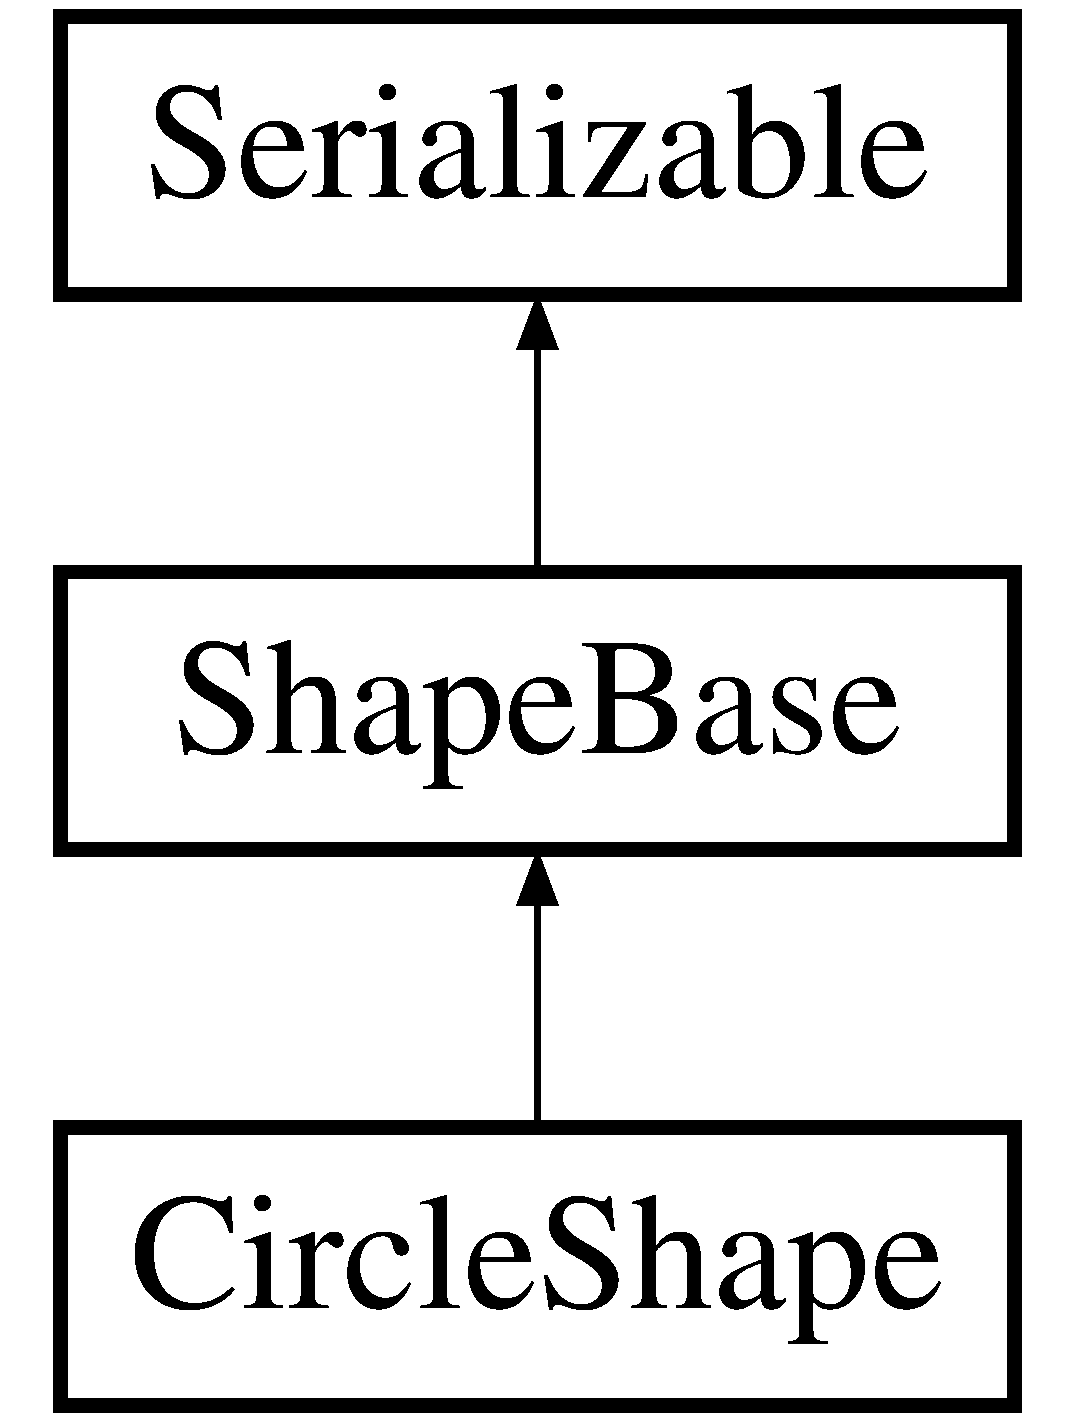
\includegraphics[height=3.000000cm]{class_circle_shape}
\end{center}
\end{figure}
\subsection*{Public Member Functions}
\begin{DoxyCompactItemize}
\item 
\textbf{ Circle\+Shape} ()
\item 
void \textbf{ set\+Dimensions} (float x, float y, float r)
\item 
void \textbf{ move} (int x, int y)
\item 
Shape \textbf{ get\+Shape} ()
\item 
boolean \textbf{ is\+Hit} (float x, float y)
\item 
void \textbf{ set\+Color} (Color new\+Color)
\item 
Color \textbf{ get\+Color} ()
\item 
void \textbf{ resize} (float value)
\end{DoxyCompactItemize}
\subsection*{Additional Inherited Members}


\subsection{Detailed Description}
Klasa odpowiedzialna za koło. \begin{DoxyAuthor}{Author}
Michał Treter 
\end{DoxyAuthor}


\subsection{Constructor \& Destructor Documentation}
\mbox{\label{class_circle_shape_a7f25499c232d3e71ce60fb94ff957aa0}} 
\index{Circle\+Shape@{Circle\+Shape}!Circle\+Shape@{Circle\+Shape}}
\index{Circle\+Shape@{Circle\+Shape}!Circle\+Shape@{Circle\+Shape}}
\subsubsection{Circle\+Shape()}
{\footnotesize\ttfamily Circle\+Shape.\+Circle\+Shape (\begin{DoxyParamCaption}{ }\end{DoxyParamCaption})}

Konstruktor klasy, nadaja kołu pusty kształt. 

\subsection{Member Function Documentation}
\mbox{\label{class_circle_shape_af3c09f8c923de5288fbf29b358edb83c}} 
\index{Circle\+Shape@{Circle\+Shape}!get\+Color@{get\+Color}}
\index{get\+Color@{get\+Color}!Circle\+Shape@{Circle\+Shape}}
\subsubsection{get\+Color()}
{\footnotesize\ttfamily Color Circle\+Shape.\+get\+Color (\begin{DoxyParamCaption}{ }\end{DoxyParamCaption})}

Metoda zwracająca kolor figury. \begin{DoxyReturn}{Returns}
Zwrócony kolor jaki figura aktualnie posiada. 
\end{DoxyReturn}
\mbox{\label{class_circle_shape_acf52c076e8572ec493865edf71d7ceee}} 
\index{Circle\+Shape@{Circle\+Shape}!get\+Shape@{get\+Shape}}
\index{get\+Shape@{get\+Shape}!Circle\+Shape@{Circle\+Shape}}
\subsubsection{get\+Shape()}
{\footnotesize\ttfamily Shape Circle\+Shape.\+get\+Shape (\begin{DoxyParamCaption}{ }\end{DoxyParamCaption})}

Metoda, która przechytuje i zwraca kształt figury. \begin{DoxyReturn}{Returns}
zwrócony kształ figury. 
\end{DoxyReturn}
\mbox{\label{class_circle_shape_ae7ab9718a4fa67def8410409e5d7934c}} 
\index{Circle\+Shape@{Circle\+Shape}!is\+Hit@{is\+Hit}}
\index{is\+Hit@{is\+Hit}!Circle\+Shape@{Circle\+Shape}}
\subsubsection{is\+Hit()}
{\footnotesize\ttfamily boolean Circle\+Shape.\+is\+Hit (\begin{DoxyParamCaption}\item[{float}]{x,  }\item[{float}]{y }\end{DoxyParamCaption})}

Metoda odpowiedzialna za sprawdzenie czy dane współrzedne znajdują sie w figurze. 
\begin{DoxyParams}{Parameters}
{\em x} & Współrzędna X kliknięcia. \\
\hline
{\em y} & Współrzędna Y kliknięcia. \\
\hline
\end{DoxyParams}
\begin{DoxyReturn}{Returns}
Wartość logiczna, prawdziwa jeśli punkty są w figurze, zaś fałyszwa w przeciwnym wypadku. 
\end{DoxyReturn}
\mbox{\label{class_circle_shape_a83c35d3d02ca6e6e982e319e2d432973}} 
\index{Circle\+Shape@{Circle\+Shape}!move@{move}}
\index{move@{move}!Circle\+Shape@{Circle\+Shape}}
\subsubsection{move()}
{\footnotesize\ttfamily void Circle\+Shape.\+move (\begin{DoxyParamCaption}\item[{int}]{x,  }\item[{int}]{y }\end{DoxyParamCaption})}

Metoda odpowiedzialna za przemieszczanie koła. 
\begin{DoxyParams}{Parameters}
{\em x} & Wartość o którą nalezy przesunąć koło w osi X. \\
\hline
{\em y} & Wartość o którą nalezy przesunąć koło w osi Y. \\
\hline
\end{DoxyParams}
\mbox{\label{class_circle_shape_a7d94c8bf4503a5ef8ea79ee0e88dc7a3}} 
\index{Circle\+Shape@{Circle\+Shape}!resize@{resize}}
\index{resize@{resize}!Circle\+Shape@{Circle\+Shape}}
\subsubsection{resize()}
{\footnotesize\ttfamily void Circle\+Shape.\+resize (\begin{DoxyParamCaption}\item[{float}]{value }\end{DoxyParamCaption})}

Metoda zmieniająca rozmiar figury. 
\begin{DoxyParams}{Parameters}
{\em value} & Wartość o jaką zostanie zwiększona figura. \\
\hline
\end{DoxyParams}
\mbox{\label{class_circle_shape_ac545acbc5f13226ebb715731db3f9a5d}} 
\index{Circle\+Shape@{Circle\+Shape}!set\+Color@{set\+Color}}
\index{set\+Color@{set\+Color}!Circle\+Shape@{Circle\+Shape}}
\subsubsection{set\+Color()}
{\footnotesize\ttfamily void Circle\+Shape.\+set\+Color (\begin{DoxyParamCaption}\item[{Color}]{new\+Color }\end{DoxyParamCaption})}

Metoda ustawiająca kolor naszej figurze. 
\begin{DoxyParams}{Parameters}
{\em new\+Color} & Nowy kolor jaki należy ustawić figurze. \\
\hline
\end{DoxyParams}
\mbox{\label{class_circle_shape_ad10715ca361cc125701d00d7046aa843}} 
\index{Circle\+Shape@{Circle\+Shape}!set\+Dimensions@{set\+Dimensions}}
\index{set\+Dimensions@{set\+Dimensions}!Circle\+Shape@{Circle\+Shape}}
\subsubsection{set\+Dimensions()}
{\footnotesize\ttfamily void Circle\+Shape.\+set\+Dimensions (\begin{DoxyParamCaption}\item[{float}]{x,  }\item[{float}]{y,  }\item[{float}]{r }\end{DoxyParamCaption})}

Metoda publiczna, której zadaniem jest ustawić rozmiar i położenie koła. 
\begin{DoxyParams}{Parameters}
{\em x} & Wartość w osi X. \\
\hline
{\em y} & Wartość w osi Y. \\
\hline
{\em r} & Wartość promienia okręgu. \\
\hline
\end{DoxyParams}


The documentation for this class was generated from the following file\+:\begin{DoxyCompactItemize}
\item 
/\+Users/\+Adimus/\+Desktop/\+N\+E\+T\+B\+I\+N\+Z/\+Geo\+Graphic\+X/src/Circle\+Shape.\+java\end{DoxyCompactItemize}

\section{Drawing\+Surface Class Reference}
\label{class_drawing_surface}\index{Drawing\+Surface@{Drawing\+Surface}}
Inheritance diagram for Drawing\+Surface\+:\begin{figure}[H]
\begin{center}
\leavevmode
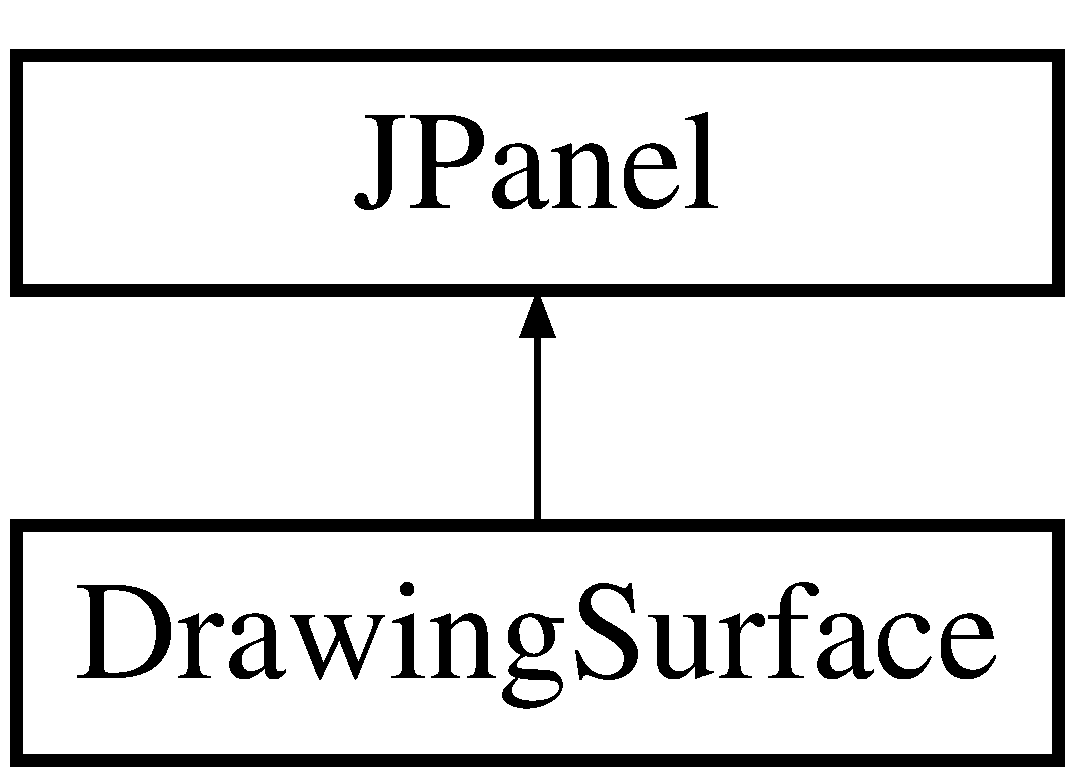
\includegraphics[height=2.000000cm]{class_drawing_surface}
\end{center}
\end{figure}
\subsection*{Public Member Functions}
\begin{DoxyCompactItemize}
\item 
\textbf{ Drawing\+Surface} (\textbf{ Geo\+GraphicX} main\+Window\+Reference)
\item 
\mbox{\label{class_drawing_surface_a5fec875fb243f233a23432403c6c3015}} 
void {\bfseries paint\+Component} (Graphics g)
\end{DoxyCompactItemize}


\subsection{Detailed Description}
Klasa generująca pole na którym będzie odbywało się rysowanie. \begin{DoxyAuthor}{Author}
Michał Treter 
\end{DoxyAuthor}


\subsection{Constructor \& Destructor Documentation}
\mbox{\label{class_drawing_surface_a7b0d154f706e1c4db872475e426f5d7a}} 
\index{Drawing\+Surface@{Drawing\+Surface}!Drawing\+Surface@{Drawing\+Surface}}
\index{Drawing\+Surface@{Drawing\+Surface}!Drawing\+Surface@{Drawing\+Surface}}
\subsubsection{Drawing\+Surface()}
{\footnotesize\ttfamily Drawing\+Surface.\+Drawing\+Surface (\begin{DoxyParamCaption}\item[{\textbf{ Geo\+GraphicX}}]{main\+Window\+Reference }\end{DoxyParamCaption})}

Konstruktor klasy, przyjmuje jako argument odwołanie do apletu. 
\begin{DoxyParams}{Parameters}
{\em main\+Window\+Reference} & \\
\hline
\end{DoxyParams}


The documentation for this class was generated from the following file\+:\begin{DoxyCompactItemize}
\item 
/\+Users/\+Adimus/\+Desktop/\+N\+E\+T\+B\+I\+N\+Z/\+Geo\+Graphic\+X/src/Drawing\+Surface.\+java\end{DoxyCompactItemize}

\section{Geo\+GraphicX Class Reference}
\label{class_geo_graphic_x}\index{Geo\+GraphicX@{Geo\+GraphicX}}
Inheritance diagram for Geo\+GraphicX\+:\begin{figure}[H]
\begin{center}
\leavevmode
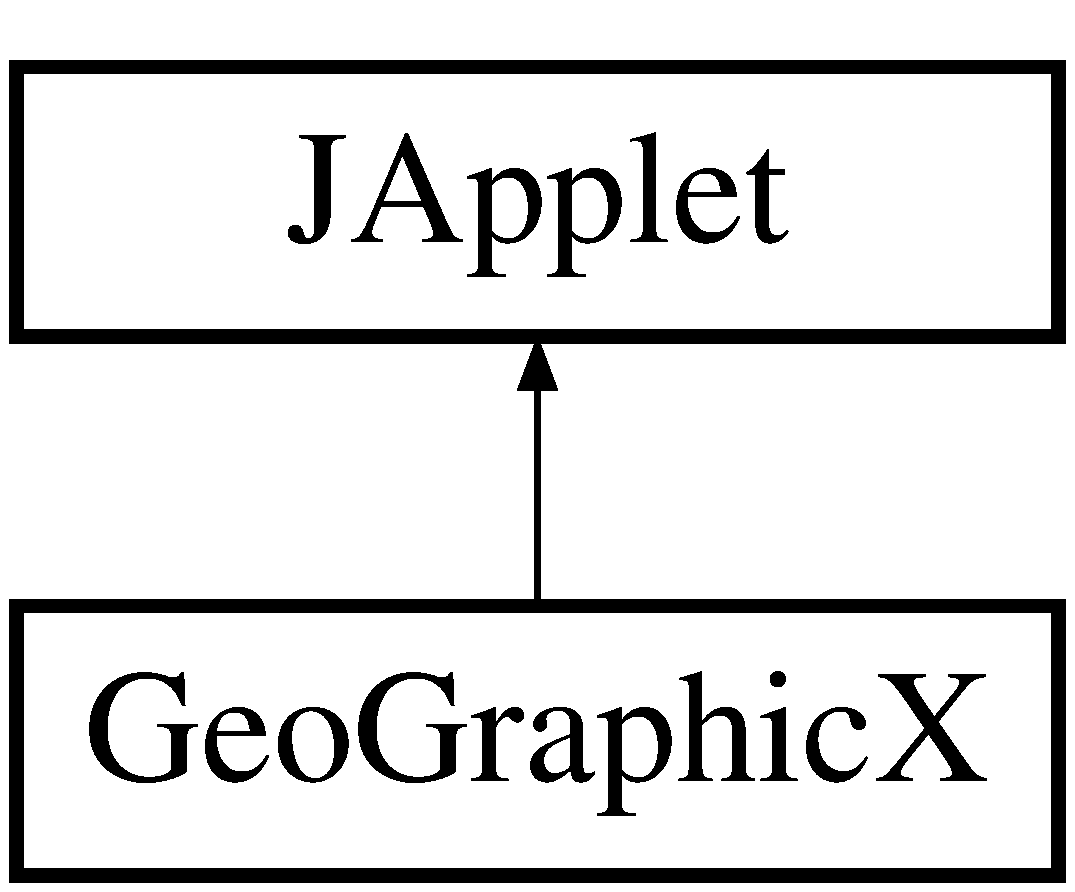
\includegraphics[height=2.000000cm]{class_geo_graphic_x}
\end{center}
\end{figure}
\subsection*{Public Member Functions}
\begin{DoxyCompactItemize}
\item 
void \textbf{ init} ()
\end{DoxyCompactItemize}
\subsection*{Static Public Member Functions}
\begin{DoxyCompactItemize}
\item 
static void \textbf{ main} (String[$\,$] args)
\end{DoxyCompactItemize}
\subsection*{Public Attributes}
\begin{DoxyCompactItemize}
\item 
boolean \textbf{ is\+Drawing\+Square} = false
\item 
boolean \textbf{ is\+Drawing\+Circle} = false
\item 
boolean \textbf{ is\+Drawing\+Poly} = false
\item 
boolean \textbf{ is\+Changing\+Color} = false
\item 
boolean \textbf{ is\+Resizing\+Figure} = false
\item 
boolean \textbf{ is\+Busy} = false
\item 
boolean \textbf{ is\+Deleting} = false
\item 
Array\+List$<$ \textbf{ Shape\+Base} $>$ \textbf{ drawable\+Objects} = new Array\+List$<$$>$()
\item 
Array\+List$<$ Shape $>$ \textbf{ temporary\+Drawable\+Objects} = new Array\+List$<$$>$()
\item 
\textbf{ temp\+Circle} \textbf{ pointer\+Circle} = new \textbf{ temp\+Circle}()
\item 
Color \textbf{ background\+Color} = new Color(255, 255, 255, 255)
\item 
\textbf{ Main\+Application\+Frame} \textbf{ main\+Frame\+Reference}
\end{DoxyCompactItemize}


\subsection{Detailed Description}
Główna klasa programu, zawiera metodę main oraz rozszerza aplet. \begin{DoxyAuthor}{Author}
Michał Treter 
\end{DoxyAuthor}


\subsection{Member Function Documentation}
\mbox{\label{class_geo_graphic_x_a8266e087ac487e55560443a44f5c87af}} 
\index{Geo\+GraphicX@{Geo\+GraphicX}!init@{init}}
\index{init@{init}!Geo\+GraphicX@{Geo\+GraphicX}}
\subsubsection{init()}
{\footnotesize\ttfamily void Geo\+Graphic\+X.\+init (\begin{DoxyParamCaption}{ }\end{DoxyParamCaption})}

Metoda inicjalizująca apletu. \mbox{\label{class_geo_graphic_x_a4cbdc0d31f6032904eae7ecb20b9fc3a}} 
\index{Geo\+GraphicX@{Geo\+GraphicX}!main@{main}}
\index{main@{main}!Geo\+GraphicX@{Geo\+GraphicX}}
\subsubsection{main()}
{\footnotesize\ttfamily static void Geo\+Graphic\+X.\+main (\begin{DoxyParamCaption}\item[{String [$\,$]}]{args }\end{DoxyParamCaption})\hspace{0.3cm}{\ttfamily [static]}}

Główna metoda main naszej aplikacji 
\begin{DoxyParams}{Parameters}
{\em args} & parametry wpisane przy uruchumieniu. \\
\hline
\end{DoxyParams}


\subsection{Member Data Documentation}
\mbox{\label{class_geo_graphic_x_a08b05acbc89547ffa879e3e1c14b03e8}} 
\index{Geo\+GraphicX@{Geo\+GraphicX}!background\+Color@{background\+Color}}
\index{background\+Color@{background\+Color}!Geo\+GraphicX@{Geo\+GraphicX}}
\subsubsection{background\+Color}
{\footnotesize\ttfamily Color Geo\+Graphic\+X.\+background\+Color = new Color(255, 255, 255, 255)}

Pole przechowujące informacjie o kolorze tła. \mbox{\label{class_geo_graphic_x_afd603afbd5712aafc94fce5071103420}} 
\index{Geo\+GraphicX@{Geo\+GraphicX}!drawable\+Objects@{drawable\+Objects}}
\index{drawable\+Objects@{drawable\+Objects}!Geo\+GraphicX@{Geo\+GraphicX}}
\subsubsection{drawable\+Objects}
{\footnotesize\ttfamily Array\+List$<$\textbf{ Shape\+Base}$>$ Geo\+Graphic\+X.\+drawable\+Objects = new Array\+List$<$$>$()}

Lista zawierająca figury do rysowania. \mbox{\label{class_geo_graphic_x_a787097390f89889774c1450be0b9b391}} 
\index{Geo\+GraphicX@{Geo\+GraphicX}!is\+Busy@{is\+Busy}}
\index{is\+Busy@{is\+Busy}!Geo\+GraphicX@{Geo\+GraphicX}}
\subsubsection{is\+Busy}
{\footnotesize\ttfamily boolean Geo\+Graphic\+X.\+is\+Busy = false}

Zmienna logiczna określająca czy jest teraz aktywny jakikolwiek proces modyfikowania figury w aplikacji. \mbox{\label{class_geo_graphic_x_a60c08c0d7db0ced8cd69b14e1cfd8043}} 
\index{Geo\+GraphicX@{Geo\+GraphicX}!is\+Changing\+Color@{is\+Changing\+Color}}
\index{is\+Changing\+Color@{is\+Changing\+Color}!Geo\+GraphicX@{Geo\+GraphicX}}
\subsubsection{is\+Changing\+Color}
{\footnotesize\ttfamily boolean Geo\+Graphic\+X.\+is\+Changing\+Color = false}

Zmienna logiczna określająca czy jest teraz aktywny proces zmiany koloru figury. \mbox{\label{class_geo_graphic_x_aad9cb8ba8a8fc82934cb0b4220ab3d72}} 
\index{Geo\+GraphicX@{Geo\+GraphicX}!is\+Deleting@{is\+Deleting}}
\index{is\+Deleting@{is\+Deleting}!Geo\+GraphicX@{Geo\+GraphicX}}
\subsubsection{is\+Deleting}
{\footnotesize\ttfamily boolean Geo\+Graphic\+X.\+is\+Deleting = false}

Zmienna logiczna określająca czy jest teraz aktywny proces usuwania figury. \mbox{\label{class_geo_graphic_x_ade4a70db318177597dd2ab2bd7982d19}} 
\index{Geo\+GraphicX@{Geo\+GraphicX}!is\+Drawing\+Circle@{is\+Drawing\+Circle}}
\index{is\+Drawing\+Circle@{is\+Drawing\+Circle}!Geo\+GraphicX@{Geo\+GraphicX}}
\subsubsection{is\+Drawing\+Circle}
{\footnotesize\ttfamily boolean Geo\+Graphic\+X.\+is\+Drawing\+Circle = false}

Zmienna logiczna określająca czy jest teraz aktywny proces ryoswania okręgu. \mbox{\label{class_geo_graphic_x_ac5d66e793eed874bcfc1883499c255f1}} 
\index{Geo\+GraphicX@{Geo\+GraphicX}!is\+Drawing\+Poly@{is\+Drawing\+Poly}}
\index{is\+Drawing\+Poly@{is\+Drawing\+Poly}!Geo\+GraphicX@{Geo\+GraphicX}}
\subsubsection{is\+Drawing\+Poly}
{\footnotesize\ttfamily boolean Geo\+Graphic\+X.\+is\+Drawing\+Poly = false}

Zmienna logiczna określająca czy jest teraz aktywny proces ryoswania wielokątu. \mbox{\label{class_geo_graphic_x_ad3bc7f2c5b0c5db882e21c5c433604ee}} 
\index{Geo\+GraphicX@{Geo\+GraphicX}!is\+Drawing\+Square@{is\+Drawing\+Square}}
\index{is\+Drawing\+Square@{is\+Drawing\+Square}!Geo\+GraphicX@{Geo\+GraphicX}}
\subsubsection{is\+Drawing\+Square}
{\footnotesize\ttfamily boolean Geo\+Graphic\+X.\+is\+Drawing\+Square = false}

Zmienna logiczna określająca czy jest teraz aktywny proces ryoswania prostokąta. \mbox{\label{class_geo_graphic_x_a0814229dbc30bdd2a5aca2b50bd258df}} 
\index{Geo\+GraphicX@{Geo\+GraphicX}!is\+Resizing\+Figure@{is\+Resizing\+Figure}}
\index{is\+Resizing\+Figure@{is\+Resizing\+Figure}!Geo\+GraphicX@{Geo\+GraphicX}}
\subsubsection{is\+Resizing\+Figure}
{\footnotesize\ttfamily boolean Geo\+Graphic\+X.\+is\+Resizing\+Figure = false}

Zmienna logiczna określająca czy jest teraz aktywny proces zmiany rozmiaru figury. \mbox{\label{class_geo_graphic_x_a199634684b043e71e078341b1c8c8989}} 
\index{Geo\+GraphicX@{Geo\+GraphicX}!main\+Frame\+Reference@{main\+Frame\+Reference}}
\index{main\+Frame\+Reference@{main\+Frame\+Reference}!Geo\+GraphicX@{Geo\+GraphicX}}
\subsubsection{main\+Frame\+Reference}
{\footnotesize\ttfamily \textbf{ Main\+Application\+Frame} Geo\+Graphic\+X.\+main\+Frame\+Reference}

Odwołanie do głównej ramki aplikacji, w której wszystko sie odbywa. \mbox{\label{class_geo_graphic_x_a9000101765183c1fb3e4a69b866cb45d}} 
\index{Geo\+GraphicX@{Geo\+GraphicX}!pointer\+Circle@{pointer\+Circle}}
\index{pointer\+Circle@{pointer\+Circle}!Geo\+GraphicX@{Geo\+GraphicX}}
\subsubsection{pointer\+Circle}
{\footnotesize\ttfamily \textbf{ temp\+Circle} Geo\+Graphic\+X.\+pointer\+Circle = new \textbf{ temp\+Circle}()}

Celownik, który pojawia się kiedy jakiś proces modyfikowania figury jest aktywny. \mbox{\label{class_geo_graphic_x_a8762800b9c7eaf083f30f7dec13921e3}} 
\index{Geo\+GraphicX@{Geo\+GraphicX}!temporary\+Drawable\+Objects@{temporary\+Drawable\+Objects}}
\index{temporary\+Drawable\+Objects@{temporary\+Drawable\+Objects}!Geo\+GraphicX@{Geo\+GraphicX}}
\subsubsection{temporary\+Drawable\+Objects}
{\footnotesize\ttfamily Array\+List$<$Shape$>$ Geo\+Graphic\+X.\+temporary\+Drawable\+Objects = new Array\+List$<$$>$()}

Lista zawierająca tymczasowe figury pomocniczne do rysowania. 

The documentation for this class was generated from the following file\+:\begin{DoxyCompactItemize}
\item 
/\+Users/\+Adimus/\+Desktop/\+N\+E\+T\+B\+I\+N\+Z/\+Geo\+Graphic\+X/src/Geo\+Graphic\+X.\+java\end{DoxyCompactItemize}

\section{Main\+Application\+Frame Class Reference}
\label{class_main_application_frame}\index{Main\+Application\+Frame@{Main\+Application\+Frame}}
Inheritance diagram for Main\+Application\+Frame\+:\begin{figure}[H]
\begin{center}
\leavevmode
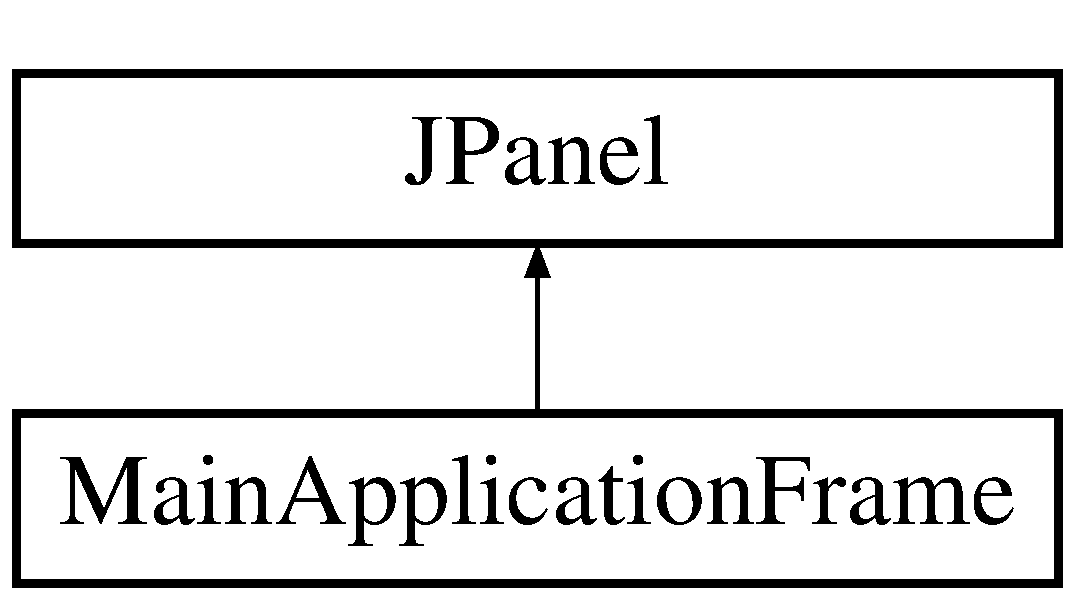
\includegraphics[height=2.000000cm]{class_main_application_frame}
\end{center}
\end{figure}
\subsection*{Public Member Functions}
\begin{DoxyCompactItemize}
\item 
\textbf{ Main\+Application\+Frame} (\textbf{ Geo\+GraphicX} main\+Applet\+Reference)
\end{DoxyCompactItemize}
\subsection*{Public Attributes}
\begin{DoxyCompactItemize}
\item 
\textbf{ Geo\+GraphicX} \textbf{ applet\+Reference}
\item 
\textbf{ Drawing\+Surface} \textbf{ draw\+Surface}
\item 
\textbf{ Operation\+Bar} \textbf{ operation\+Bar}
\end{DoxyCompactItemize}


\subsection{Detailed Description}
Klasa w której generowana jest główna ramka aplikacji. \begin{DoxyAuthor}{Author}
Michał Treter 
\end{DoxyAuthor}


\subsection{Constructor \& Destructor Documentation}
\mbox{\label{class_main_application_frame_ad5f2f19159866db4d1ba182ea437da8e}} 
\index{Main\+Application\+Frame@{Main\+Application\+Frame}!Main\+Application\+Frame@{Main\+Application\+Frame}}
\index{Main\+Application\+Frame@{Main\+Application\+Frame}!Main\+Application\+Frame@{Main\+Application\+Frame}}
\subsubsection{Main\+Application\+Frame()}
{\footnotesize\ttfamily Main\+Application\+Frame.\+Main\+Application\+Frame (\begin{DoxyParamCaption}\item[{\textbf{ Geo\+GraphicX}}]{main\+Applet\+Reference }\end{DoxyParamCaption})}

Konstruktor naszej klasy. 
\begin{DoxyParams}{Parameters}
{\em main\+Applet\+Reference} & Odwołanie do apletu, z którego został wywołany konstruktor. \\
\hline
\end{DoxyParams}


\subsection{Member Data Documentation}
\mbox{\label{class_main_application_frame_a505141826249708171cf2ef393051c2c}} 
\index{Main\+Application\+Frame@{Main\+Application\+Frame}!applet\+Reference@{applet\+Reference}}
\index{applet\+Reference@{applet\+Reference}!Main\+Application\+Frame@{Main\+Application\+Frame}}
\subsubsection{applet\+Reference}
{\footnotesize\ttfamily \textbf{ Geo\+GraphicX} Main\+Application\+Frame.\+applet\+Reference}

Odwołanie do głównej klasy. \mbox{\label{class_main_application_frame_a1a94fccde37da6545ea39c9f290f82b0}} 
\index{Main\+Application\+Frame@{Main\+Application\+Frame}!draw\+Surface@{draw\+Surface}}
\index{draw\+Surface@{draw\+Surface}!Main\+Application\+Frame@{Main\+Application\+Frame}}
\subsubsection{draw\+Surface}
{\footnotesize\ttfamily \textbf{ Drawing\+Surface} Main\+Application\+Frame.\+draw\+Surface}

Odwoałanie do przestrzeni do rysowania. \mbox{\label{class_main_application_frame_a8c7a1cc5cd71aa5f3af8c8e045877bdb}} 
\index{Main\+Application\+Frame@{Main\+Application\+Frame}!operation\+Bar@{operation\+Bar}}
\index{operation\+Bar@{operation\+Bar}!Main\+Application\+Frame@{Main\+Application\+Frame}}
\subsubsection{operation\+Bar}
{\footnotesize\ttfamily \textbf{ Operation\+Bar} Main\+Application\+Frame.\+operation\+Bar}

Odwołanie do panelu operacji. 

The documentation for this class was generated from the following file\+:\begin{DoxyCompactItemize}
\item 
/\+Users/\+Adimus/\+Desktop/\+N\+E\+T\+B\+I\+N\+Z/\+Geo\+Graphic\+X/src/Main\+Application\+Frame.\+java\end{DoxyCompactItemize}

\section{Main\+Menu Class Reference}
\label{class_main_menu}\index{Main\+Menu@{Main\+Menu}}
Inheritance diagram for Main\+Menu\+:\begin{figure}[H]
\begin{center}
\leavevmode
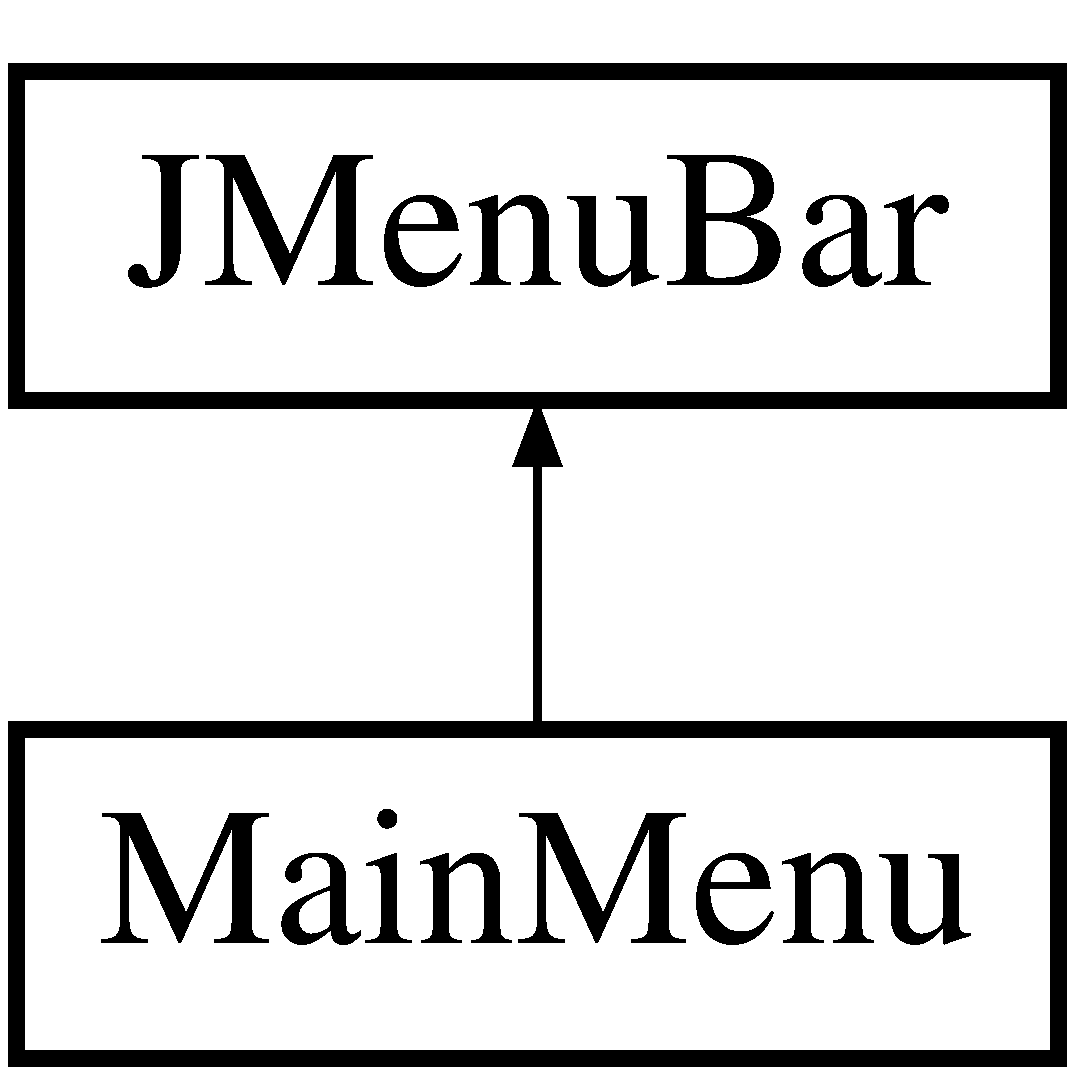
\includegraphics[height=2.000000cm]{class_main_menu}
\end{center}
\end{figure}
\subsection*{Public Member Functions}
\begin{DoxyCompactItemize}
\item 
\textbf{ Main\+Menu} (\textbf{ Geo\+GraphicX} main\+Window\+Reference)
\end{DoxyCompactItemize}


\subsection{Detailed Description}
Klasa, która jest odpowiedzialna za pasek menu. \begin{DoxyAuthor}{Author}
Michał Treter 
\end{DoxyAuthor}


\subsection{Constructor \& Destructor Documentation}
\mbox{\label{class_main_menu_a95fdb1f3b86e3ef7ecc382534ff644b7}} 
\index{Main\+Menu@{Main\+Menu}!Main\+Menu@{Main\+Menu}}
\index{Main\+Menu@{Main\+Menu}!Main\+Menu@{Main\+Menu}}
\subsubsection{Main\+Menu()}
{\footnotesize\ttfamily Main\+Menu.\+Main\+Menu (\begin{DoxyParamCaption}\item[{\textbf{ Geo\+GraphicX}}]{main\+Window\+Reference }\end{DoxyParamCaption})}

Konstuktor klasy, w którym są tworzone pozycje do paska menu oraz dodawane. W nim także każdy element dostaje swoją akcję. 
\begin{DoxyParams}{Parameters}
{\em main\+Window\+Reference} & Odwołanie do głównego apletu. \\
\hline
\end{DoxyParams}


The documentation for this class was generated from the following file\+:\begin{DoxyCompactItemize}
\item 
/\+Users/\+Adimus/\+Desktop/\+N\+E\+T\+B\+I\+N\+Z/\+Geo\+Graphic\+X/src/Main\+Menu.\+java\end{DoxyCompactItemize}

\section{Mouse\+Operation\+Controller Class Reference}
\label{class_mouse_operation_controller}\index{Mouse\+Operation\+Controller@{Mouse\+Operation\+Controller}}
Inheritance diagram for Mouse\+Operation\+Controller\+:\begin{figure}[H]
\begin{center}
\leavevmode
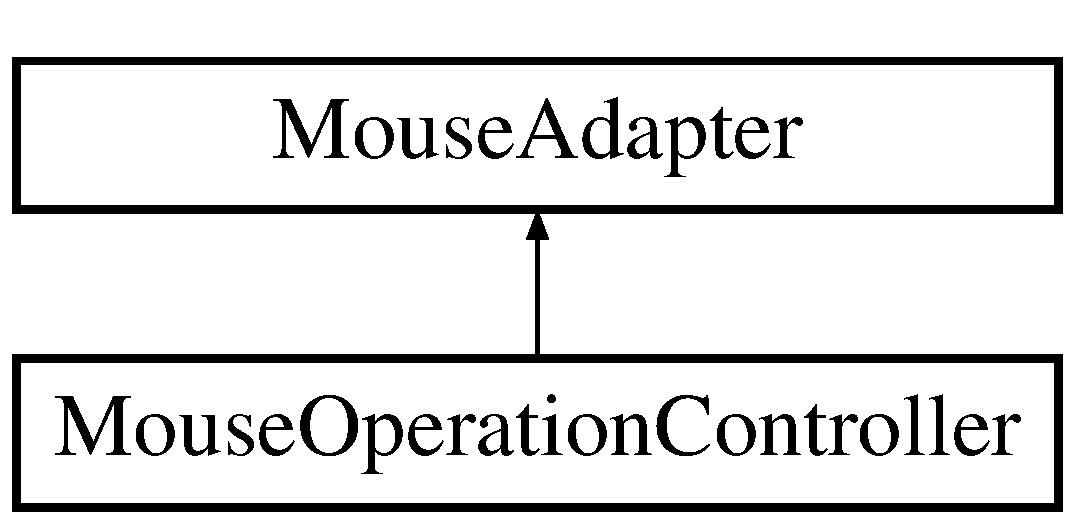
\includegraphics[height=2.000000cm]{class_mouse_operation_controller}
\end{center}
\end{figure}
\subsection*{Public Member Functions}
\begin{DoxyCompactItemize}
\item 
\textbf{ Mouse\+Operation\+Controller} (\textbf{ Geo\+GraphicX} main\+Window\+Reference)
\item 
\mbox{\label{class_mouse_operation_controller_abd98fc9952b8cade251559655074e18f}} 
void {\bfseries mouse\+Moved} (Mouse\+Event e)
\item 
\mbox{\label{class_mouse_operation_controller_ae75e28891a828d5572a66d432d5614af}} 
void {\bfseries mouse\+Exited} (Mouse\+Event e)
\item 
\mbox{\label{class_mouse_operation_controller_aa899611e53870726b21b860eade6a209}} 
void {\bfseries mouse\+Dragged} (Mouse\+Event e)
\item 
\mbox{\label{class_mouse_operation_controller_acf59899ca44f8be7483af10919668b1f}} 
void {\bfseries mouse\+Released} (Mouse\+Event e)
\item 
\mbox{\label{class_mouse_operation_controller_ab87e47fbe4711dd9ea2abb300ae24af0}} 
void {\bfseries mouse\+Clicked} (Mouse\+Event e)
\end{DoxyCompactItemize}
\subsection*{Public Attributes}
\begin{DoxyCompactItemize}
\item 
int \textbf{ hit\+Index} = -\/1
\end{DoxyCompactItemize}


\subsection{Detailed Description}
Klasa odpowiedzialna za kontrole ruchów oraz kliknięć myszy. W klasie tej także zawarta jest cała logika programu oraz tego jak należy wykonywać poszczególne operacje na poszczególnych figurach, oraz nadzoruje proces tworzenia nowych figur i usuwania wybranych. \begin{DoxyAuthor}{Author}
Michał Treter 
\end{DoxyAuthor}


\subsection{Constructor \& Destructor Documentation}
\mbox{\label{class_mouse_operation_controller_ae6f41a249d5256fd714c9a3a706d9f3b}} 
\index{Mouse\+Operation\+Controller@{Mouse\+Operation\+Controller}!Mouse\+Operation\+Controller@{Mouse\+Operation\+Controller}}
\index{Mouse\+Operation\+Controller@{Mouse\+Operation\+Controller}!Mouse\+Operation\+Controller@{Mouse\+Operation\+Controller}}
\subsubsection{Mouse\+Operation\+Controller()}
{\footnotesize\ttfamily Mouse\+Operation\+Controller.\+Mouse\+Operation\+Controller (\begin{DoxyParamCaption}\item[{\textbf{ Geo\+GraphicX}}]{main\+Window\+Reference }\end{DoxyParamCaption})}

Konstruktor naszej klasy. 
\begin{DoxyParams}{Parameters}
{\em main\+Window\+Reference} & Odwołanie do głównego apletu. \\
\hline
\end{DoxyParams}


\subsection{Member Data Documentation}
\mbox{\label{class_mouse_operation_controller_a2f1af5997db6cd521699d2eca5eea946}} 
\index{Mouse\+Operation\+Controller@{Mouse\+Operation\+Controller}!hit\+Index@{hit\+Index}}
\index{hit\+Index@{hit\+Index}!Mouse\+Operation\+Controller@{Mouse\+Operation\+Controller}}
\subsubsection{hit\+Index}
{\footnotesize\ttfamily int Mouse\+Operation\+Controller.\+hit\+Index = -\/1}

Zmienna przechowująca numer figury z listy, która został kliknięty. 

The documentation for this class was generated from the following file\+:\begin{DoxyCompactItemize}
\item 
/\+Users/\+Adimus/\+Desktop/\+N\+E\+T\+B\+I\+N\+Z/\+Geo\+Graphic\+X/src/Mouse\+Operation\+Controller.\+java\end{DoxyCompactItemize}

\section{Operation\+Bar Class Reference}
\label{class_operation_bar}\index{Operation\+Bar@{Operation\+Bar}}
Inheritance diagram for Operation\+Bar\+:\begin{figure}[H]
\begin{center}
\leavevmode
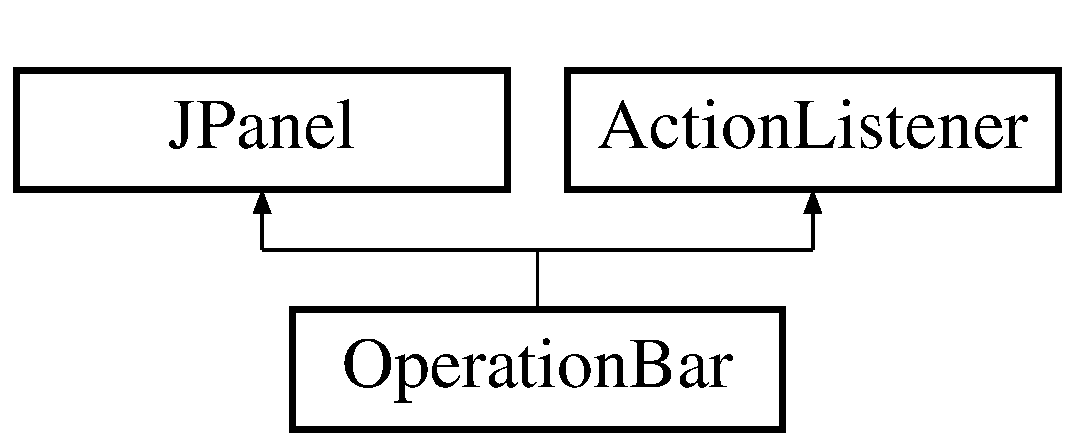
\includegraphics[height=2.000000cm]{class_operation_bar}
\end{center}
\end{figure}
\subsection*{Public Member Functions}
\begin{DoxyCompactItemize}
\item 
\textbf{ Operation\+Bar} (\textbf{ Geo\+GraphicX} main\+Window\+Reference)
\item 
\mbox{\label{class_operation_bar_a7030a65ba82068ab50bb059131ee8e05}} 
void {\bfseries paint\+Component} (Graphics g)
\item 
\mbox{\label{class_operation_bar_a0630107254ce3d8ca3845a4b885e89e2}} 
void {\bfseries action\+Performed} (Action\+Event e)
\end{DoxyCompactItemize}
\subsection*{Public Attributes}
\begin{DoxyCompactItemize}
\item 
\textbf{ Geo\+GraphicX} \textbf{ applet\+Reference}
\item 
J\+Button \textbf{ add\+Rect}
\item 
J\+Button \textbf{ add\+Circle}
\item 
J\+Button \textbf{ add\+Poly}
\item 
J\+Button \textbf{ resize\+Action}
\item 
J\+Button \textbf{ color\+Change\+Action}
\item 
J\+Button \textbf{ delete\+Action}
\item 
J\+Button \textbf{ change\+Background\+Action}
\end{DoxyCompactItemize}


\subsection{Detailed Description}
Klasa zawierająca pasek operacji. \begin{DoxyAuthor}{Author}
Michał Treter 
\end{DoxyAuthor}


\subsection{Constructor \& Destructor Documentation}
\mbox{\label{class_operation_bar_a00afa9dcb2820a68ccfce0071c34a4b2}} 
\index{Operation\+Bar@{Operation\+Bar}!Operation\+Bar@{Operation\+Bar}}
\index{Operation\+Bar@{Operation\+Bar}!Operation\+Bar@{Operation\+Bar}}
\subsubsection{Operation\+Bar()}
{\footnotesize\ttfamily Operation\+Bar.\+Operation\+Bar (\begin{DoxyParamCaption}\item[{\textbf{ Geo\+GraphicX}}]{main\+Window\+Reference }\end{DoxyParamCaption})}

Kontruktor klasy w, którym zostaję stworzony każdy z przycisków następnie każdemu z nich zostaje przypisana akcja. Na koniec przyciski zostają dodane do jednego panelu. 
\begin{DoxyParams}{Parameters}
{\em main\+Window\+Reference} & Odwołanie do głównego apletu. \\
\hline
\end{DoxyParams}


\subsection{Member Data Documentation}
\mbox{\label{class_operation_bar_a367705a6fa8dfdf841bccd5034a69653}} 
\index{Operation\+Bar@{Operation\+Bar}!add\+Circle@{add\+Circle}}
\index{add\+Circle@{add\+Circle}!Operation\+Bar@{Operation\+Bar}}
\subsubsection{add\+Circle}
{\footnotesize\ttfamily J\+Button Operation\+Bar.\+add\+Circle}

Przycisk dodawania okręgu. \mbox{\label{class_operation_bar_a4ac995bc8e8fa0d196b856847b158a2b}} 
\index{Operation\+Bar@{Operation\+Bar}!add\+Poly@{add\+Poly}}
\index{add\+Poly@{add\+Poly}!Operation\+Bar@{Operation\+Bar}}
\subsubsection{add\+Poly}
{\footnotesize\ttfamily J\+Button Operation\+Bar.\+add\+Poly}

Przycisk dodawania wielokątu. \mbox{\label{class_operation_bar_a33cae877bb167029955491e1319d1f57}} 
\index{Operation\+Bar@{Operation\+Bar}!add\+Rect@{add\+Rect}}
\index{add\+Rect@{add\+Rect}!Operation\+Bar@{Operation\+Bar}}
\subsubsection{add\+Rect}
{\footnotesize\ttfamily J\+Button Operation\+Bar.\+add\+Rect}

Przycisk dodawania prostokąta. \mbox{\label{class_operation_bar_a685ead7341a7cef4b79af4a980b640ca}} 
\index{Operation\+Bar@{Operation\+Bar}!applet\+Reference@{applet\+Reference}}
\index{applet\+Reference@{applet\+Reference}!Operation\+Bar@{Operation\+Bar}}
\subsubsection{applet\+Reference}
{\footnotesize\ttfamily \textbf{ Geo\+GraphicX} Operation\+Bar.\+applet\+Reference}

Odwołanie do głównego apletu. \mbox{\label{class_operation_bar_afef0595de60802e174541fbf7d25059f}} 
\index{Operation\+Bar@{Operation\+Bar}!change\+Background\+Action@{change\+Background\+Action}}
\index{change\+Background\+Action@{change\+Background\+Action}!Operation\+Bar@{Operation\+Bar}}
\subsubsection{change\+Background\+Action}
{\footnotesize\ttfamily J\+Button Operation\+Bar.\+change\+Background\+Action}

Przycisk aktywujący akcję zmiany koloru tła. \mbox{\label{class_operation_bar_ae834010488359b6eaf8246d604ead9f2}} 
\index{Operation\+Bar@{Operation\+Bar}!color\+Change\+Action@{color\+Change\+Action}}
\index{color\+Change\+Action@{color\+Change\+Action}!Operation\+Bar@{Operation\+Bar}}
\subsubsection{color\+Change\+Action}
{\footnotesize\ttfamily J\+Button Operation\+Bar.\+color\+Change\+Action}

Przycisk aktywujący akcje zmiany koloru figury. \mbox{\label{class_operation_bar_ac099d8aed8f41bdef2a28e4356ec2063}} 
\index{Operation\+Bar@{Operation\+Bar}!delete\+Action@{delete\+Action}}
\index{delete\+Action@{delete\+Action}!Operation\+Bar@{Operation\+Bar}}
\subsubsection{delete\+Action}
{\footnotesize\ttfamily J\+Button Operation\+Bar.\+delete\+Action}

Przycisk aktywujący akcję usuwania figury. \mbox{\label{class_operation_bar_a590fd08e1dd712cc1494cd9c6a5f0694}} 
\index{Operation\+Bar@{Operation\+Bar}!resize\+Action@{resize\+Action}}
\index{resize\+Action@{resize\+Action}!Operation\+Bar@{Operation\+Bar}}
\subsubsection{resize\+Action}
{\footnotesize\ttfamily J\+Button Operation\+Bar.\+resize\+Action}

Przycisk aktywujący akcję zmiany rozmiaru figury. 

The documentation for this class was generated from the following file\+:\begin{DoxyCompactItemize}
\item 
/\+Users/\+Adimus/\+Desktop/\+N\+E\+T\+B\+I\+N\+Z/\+Geo\+Graphic\+X/src/Operation\+Bar.\+java\end{DoxyCompactItemize}

\section{Poly\+Shape Class Reference}
\label{class_poly_shape}\index{Poly\+Shape@{Poly\+Shape}}
Inheritance diagram for Poly\+Shape\+:\begin{figure}[H]
\begin{center}
\leavevmode
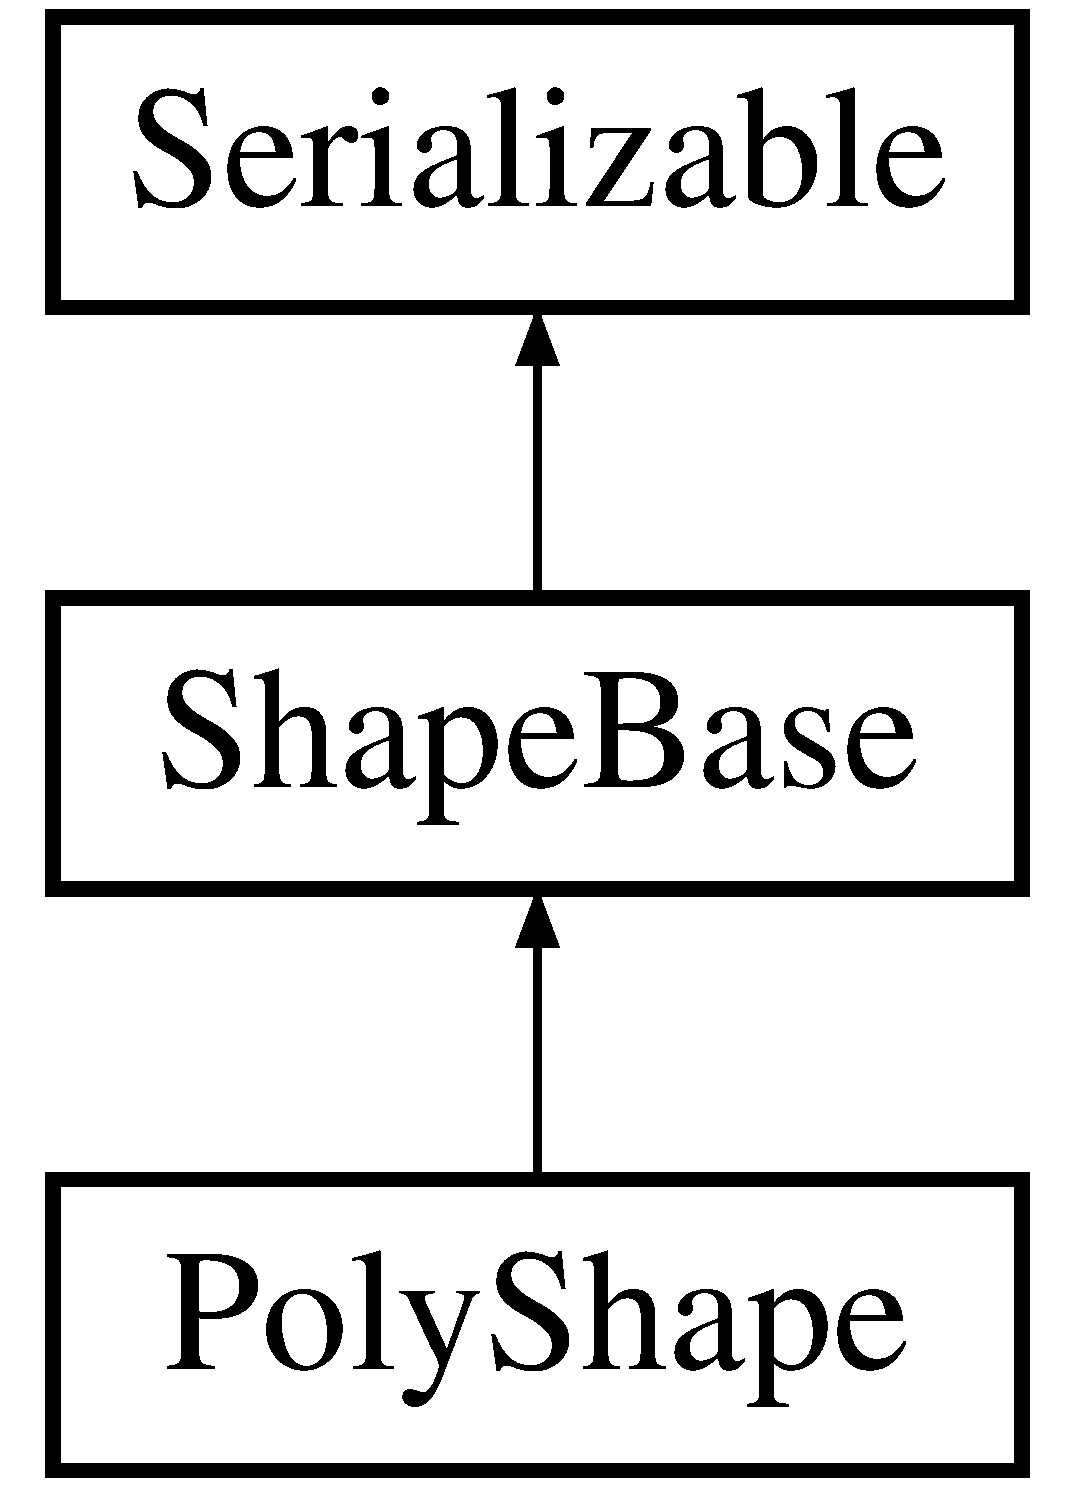
\includegraphics[height=3.000000cm]{class_poly_shape}
\end{center}
\end{figure}
\subsection*{Public Member Functions}
\begin{DoxyCompactItemize}
\item 
\textbf{ Poly\+Shape} ()
\item 
void \textbf{ set\+Dimensions} (Array\+List$<$ Point $>$ points\+List)
\item 
void \textbf{ move} (int x, int y)
\item 
Shape \textbf{ get\+Shape} ()
\item 
boolean \textbf{ is\+Hit} (float x, float y)
\item 
void \textbf{ set\+Color} (Color new\+Color)
\item 
Color \textbf{ get\+Color} ()
\item 
void \textbf{ resize} (float value)
\end{DoxyCompactItemize}
\subsection*{Protected Attributes}
\begin{DoxyCompactItemize}
\item 
Polygon \textbf{ poly\+Shape}
\item 
float \textbf{ centerX}
\end{DoxyCompactItemize}


\subsection{Detailed Description}
Klasa odpowiedzialna za wielokąt. \begin{DoxyAuthor}{Author}
Michał Treter 
\end{DoxyAuthor}


\subsection{Constructor \& Destructor Documentation}
\mbox{\label{class_poly_shape_a1ac35b96be61a45c324792ed1cbd2463}} 
\index{Poly\+Shape@{Poly\+Shape}!Poly\+Shape@{Poly\+Shape}}
\index{Poly\+Shape@{Poly\+Shape}!Poly\+Shape@{Poly\+Shape}}
\subsubsection{Poly\+Shape()}
{\footnotesize\ttfamily Poly\+Shape.\+Poly\+Shape (\begin{DoxyParamCaption}{ }\end{DoxyParamCaption})}

Konstuktor klasy. Przypisuje pusty wielokąt. 

\subsection{Member Function Documentation}
\mbox{\label{class_poly_shape_adc6cbbc34dfdc5cdf492697378baee96}} 
\index{Poly\+Shape@{Poly\+Shape}!get\+Color@{get\+Color}}
\index{get\+Color@{get\+Color}!Poly\+Shape@{Poly\+Shape}}
\subsubsection{get\+Color()}
{\footnotesize\ttfamily Color Poly\+Shape.\+get\+Color (\begin{DoxyParamCaption}{ }\end{DoxyParamCaption})}

Metoda zwracjąca akutalny kolor figury. \begin{DoxyReturn}{Returns}
aktualny kolor figury. 
\end{DoxyReturn}
\mbox{\label{class_poly_shape_a76f38be1401146e9d7d29e7fcc352e35}} 
\index{Poly\+Shape@{Poly\+Shape}!get\+Shape@{get\+Shape}}
\index{get\+Shape@{get\+Shape}!Poly\+Shape@{Poly\+Shape}}
\subsubsection{get\+Shape()}
{\footnotesize\ttfamily Shape Poly\+Shape.\+get\+Shape (\begin{DoxyParamCaption}{ }\end{DoxyParamCaption})}

Metoda zwracająca kształt figury. \begin{DoxyReturn}{Returns}
Kształ wielokątu. 
\end{DoxyReturn}
\mbox{\label{class_poly_shape_ae38333d9b47fd540e8f5c16ba285627a}} 
\index{Poly\+Shape@{Poly\+Shape}!is\+Hit@{is\+Hit}}
\index{is\+Hit@{is\+Hit}!Poly\+Shape@{Poly\+Shape}}
\subsubsection{is\+Hit()}
{\footnotesize\ttfamily boolean Poly\+Shape.\+is\+Hit (\begin{DoxyParamCaption}\item[{float}]{x,  }\item[{float}]{y }\end{DoxyParamCaption})}

Metoda odpowiedzialna za sprawdzenie czy dane współrzedne znajdują sie w figurze. 
\begin{DoxyParams}{Parameters}
{\em x} & Współrzędna X kliknięcia. \\
\hline
{\em y} & Współrzędna Y kliknięcia. \\
\hline
\end{DoxyParams}
\begin{DoxyReturn}{Returns}
Wartość logiczna, prawdziwa jeśli punkty są w figurze, zaś fałyszwa w przeciwnym wypadku. 
\end{DoxyReturn}
\mbox{\label{class_poly_shape_a8e0760e4b7e078bd5db185f5c09c7158}} 
\index{Poly\+Shape@{Poly\+Shape}!move@{move}}
\index{move@{move}!Poly\+Shape@{Poly\+Shape}}
\subsubsection{move()}
{\footnotesize\ttfamily void Poly\+Shape.\+move (\begin{DoxyParamCaption}\item[{int}]{x,  }\item[{int}]{y }\end{DoxyParamCaption})}

Metoda przesuwająca wielokąt w osi X i osi Y. 
\begin{DoxyParams}{Parameters}
{\em x} & Wartość o jaką należy przesunąć figurę w osi X. \\
\hline
{\em y} & Wartość o jaką należy przesunąć figurę w osi Y. \\
\hline
\end{DoxyParams}
\mbox{\label{class_poly_shape_ae62899d2851dbd8156b9d4162807fe30}} 
\index{Poly\+Shape@{Poly\+Shape}!resize@{resize}}
\index{resize@{resize}!Poly\+Shape@{Poly\+Shape}}
\subsubsection{resize()}
{\footnotesize\ttfamily void Poly\+Shape.\+resize (\begin{DoxyParamCaption}\item[{float}]{value }\end{DoxyParamCaption})}

Metoda zmieniająca rozmiar figur. 
\begin{DoxyParams}{Parameters}
{\em value} & Wartość o jaką należy zmienić rozmiar figury. \\
\hline
\end{DoxyParams}
\mbox{\label{class_poly_shape_a040120940c2e88f61aa83b475143a5db}} 
\index{Poly\+Shape@{Poly\+Shape}!set\+Color@{set\+Color}}
\index{set\+Color@{set\+Color}!Poly\+Shape@{Poly\+Shape}}
\subsubsection{set\+Color()}
{\footnotesize\ttfamily void Poly\+Shape.\+set\+Color (\begin{DoxyParamCaption}\item[{Color}]{new\+Color }\end{DoxyParamCaption})}

Metoda ustawiająca figurze nowy kolor. 
\begin{DoxyParams}{Parameters}
{\em new\+Color} & Nowy kolor. \\
\hline
\end{DoxyParams}
\mbox{\label{class_poly_shape_ad726002d0715c48fb3170d217c2776b8}} 
\index{Poly\+Shape@{Poly\+Shape}!set\+Dimensions@{set\+Dimensions}}
\index{set\+Dimensions@{set\+Dimensions}!Poly\+Shape@{Poly\+Shape}}
\subsubsection{set\+Dimensions()}
{\footnotesize\ttfamily void Poly\+Shape.\+set\+Dimensions (\begin{DoxyParamCaption}\item[{Array\+List$<$ Point $>$}]{points\+List }\end{DoxyParamCaption})}

Metoda ustawiająca pozycje oraz rozmiar wielokątu poprzez dodawanie punktów do jego struktury. 
\begin{DoxyParams}{Parameters}
{\em points\+List} & \\
\hline
\end{DoxyParams}


\subsection{Member Data Documentation}
\mbox{\label{class_poly_shape_a651a20eeb881b58cd9f55aa63e9a859c}} 
\index{Poly\+Shape@{Poly\+Shape}!centerX@{centerX}}
\index{centerX@{centerX}!Poly\+Shape@{Poly\+Shape}}
\subsubsection{centerX}
{\footnotesize\ttfamily float Poly\+Shape.\+centerX\hspace{0.3cm}{\ttfamily [protected]}}

Zmienna zawierjąca X środka figury. \mbox{\label{class_poly_shape_a7115455fc518afe762f1aba1078ff4b2}} 
\index{Poly\+Shape@{Poly\+Shape}!poly\+Shape@{poly\+Shape}}
\index{poly\+Shape@{poly\+Shape}!Poly\+Shape@{Poly\+Shape}}
\subsubsection{poly\+Shape}
{\footnotesize\ttfamily Polygon Poly\+Shape.\+poly\+Shape\hspace{0.3cm}{\ttfamily [protected]}}

Kształt wielokątu. 

The documentation for this class was generated from the following file\+:\begin{DoxyCompactItemize}
\item 
/\+Users/\+Adimus/\+Desktop/\+N\+E\+T\+B\+I\+N\+Z/\+Geo\+Graphic\+X/src/Poly\+Shape.\+java\end{DoxyCompactItemize}

\section{Rect\+Shape Class Reference}
\label{class_rect_shape}\index{Rect\+Shape@{Rect\+Shape}}
Inheritance diagram for Rect\+Shape\+:\begin{figure}[H]
\begin{center}
\leavevmode
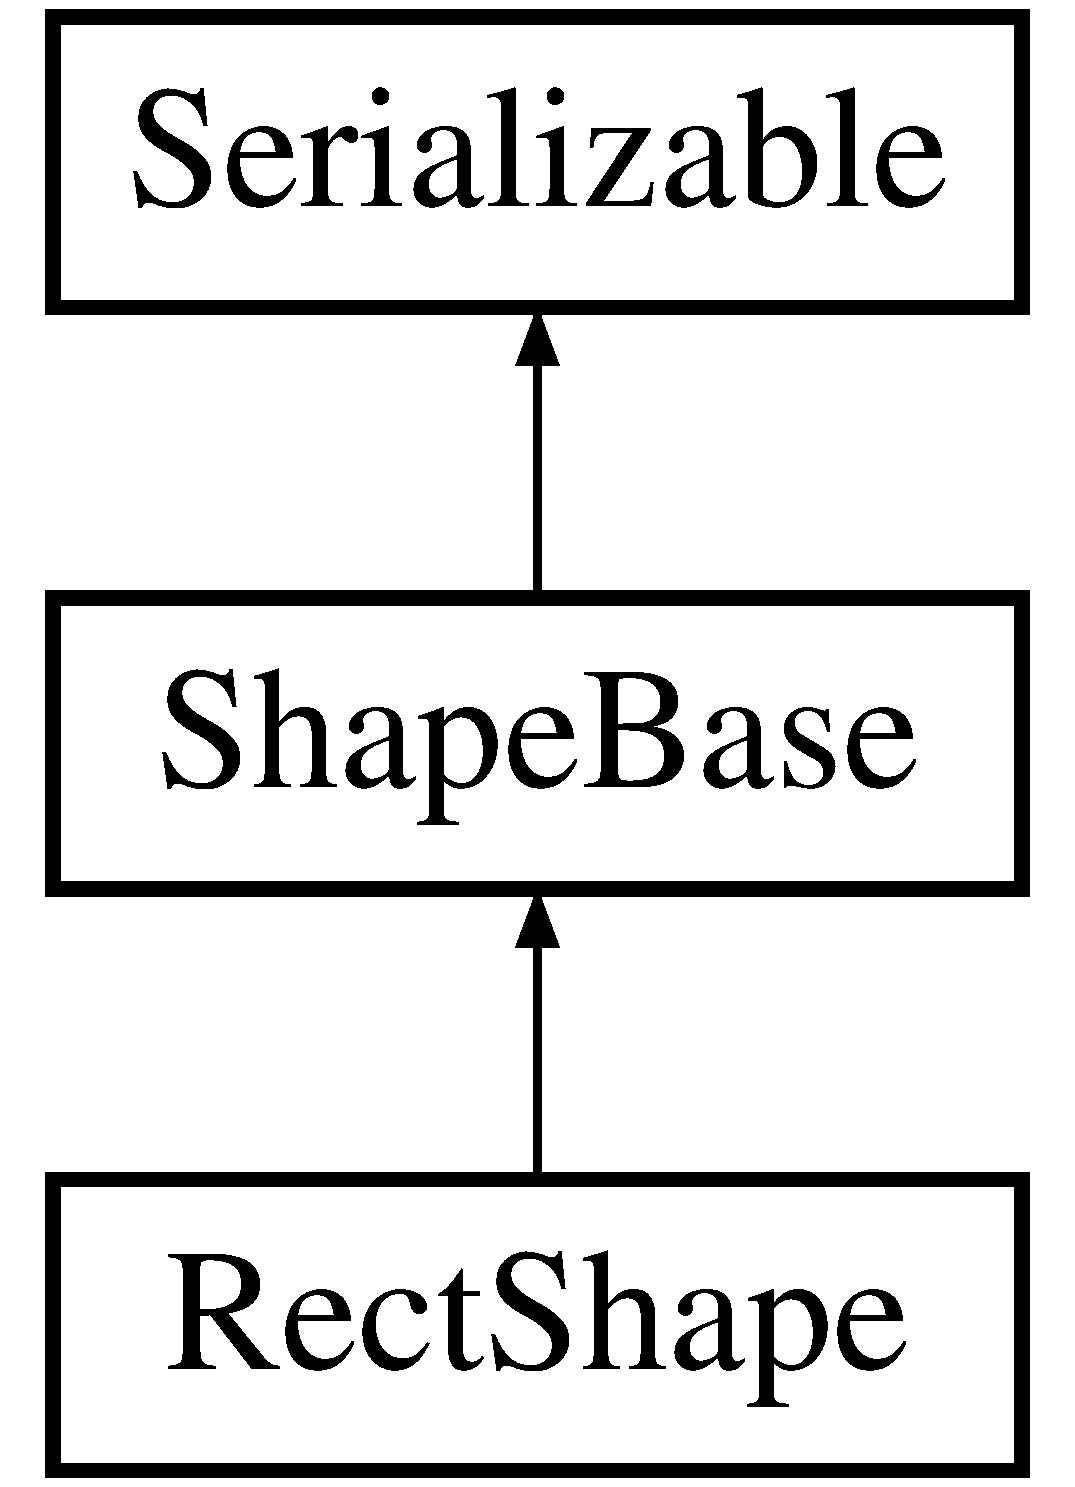
\includegraphics[height=3.000000cm]{class_rect_shape}
\end{center}
\end{figure}
\subsection*{Public Member Functions}
\begin{DoxyCompactItemize}
\item 
\textbf{ Rect\+Shape} ()
\item 
void \textbf{ set\+Dimensions} (float x, float y, float width, float height)
\item 
void \textbf{ move} (int x, int y)
\item 
Shape \textbf{ get\+Shape} ()
\item 
void \textbf{ set\+Color} (Color new\+Color)
\item 
boolean \textbf{ is\+Hit} (float x, float y)
\item 
Color \textbf{ get\+Color} ()
\item 
void \textbf{ resize} (float value)
\end{DoxyCompactItemize}
\subsection*{Protected Attributes}
\begin{DoxyCompactItemize}
\item 
Rectangle2\+D.\+Float \textbf{ shape\+Of\+Figure} = new Rectangle2\+D.\+Float()
\end{DoxyCompactItemize}


\subsection{Detailed Description}
Klasa odpowiedzialna za prostokąt. \begin{DoxyAuthor}{Author}
Michał Treter 
\end{DoxyAuthor}


\subsection{Constructor \& Destructor Documentation}
\mbox{\label{class_rect_shape_a86cf01c77c39a2052a3706747c9ae27e}} 
\index{Rect\+Shape@{Rect\+Shape}!Rect\+Shape@{Rect\+Shape}}
\index{Rect\+Shape@{Rect\+Shape}!Rect\+Shape@{Rect\+Shape}}
\subsubsection{Rect\+Shape()}
{\footnotesize\ttfamily Rect\+Shape.\+Rect\+Shape (\begin{DoxyParamCaption}{ }\end{DoxyParamCaption})}

Konstruktor klasy, zeruje kształt prostokątu. 

\subsection{Member Function Documentation}
\mbox{\label{class_rect_shape_a313190c5754f9d952657f3234cbc50ff}} 
\index{Rect\+Shape@{Rect\+Shape}!get\+Color@{get\+Color}}
\index{get\+Color@{get\+Color}!Rect\+Shape@{Rect\+Shape}}
\subsubsection{get\+Color()}
{\footnotesize\ttfamily Color Rect\+Shape.\+get\+Color (\begin{DoxyParamCaption}{ }\end{DoxyParamCaption})}

Metoda zwracjąca akutalny kolor figury. \begin{DoxyReturn}{Returns}
aktualny kolor figury. 
\end{DoxyReturn}
\mbox{\label{class_rect_shape_ae9313879935fedaa1a1f881fbab9b9cf}} 
\index{Rect\+Shape@{Rect\+Shape}!get\+Shape@{get\+Shape}}
\index{get\+Shape@{get\+Shape}!Rect\+Shape@{Rect\+Shape}}
\subsubsection{get\+Shape()}
{\footnotesize\ttfamily Shape Rect\+Shape.\+get\+Shape (\begin{DoxyParamCaption}{ }\end{DoxyParamCaption})}

Metoda zwracająca kształt figury. \begin{DoxyReturn}{Returns}
Kształ prostokątu. 
\end{DoxyReturn}
\mbox{\label{class_rect_shape_a326606d5a71b40cb81324c9222f341e0}} 
\index{Rect\+Shape@{Rect\+Shape}!is\+Hit@{is\+Hit}}
\index{is\+Hit@{is\+Hit}!Rect\+Shape@{Rect\+Shape}}
\subsubsection{is\+Hit()}
{\footnotesize\ttfamily boolean Rect\+Shape.\+is\+Hit (\begin{DoxyParamCaption}\item[{float}]{x,  }\item[{float}]{y }\end{DoxyParamCaption})}

Metoda odpowiedzialna za sprawdzenie czy dane współrzedne znajdują sie w figurze. 
\begin{DoxyParams}{Parameters}
{\em x} & Współrzędna X kliknięcia. \\
\hline
{\em y} & Współrzędna Y kliknięcia. \\
\hline
\end{DoxyParams}
\begin{DoxyReturn}{Returns}
Wartość logiczna, prawdziwa jeśli punkty są w figurze, zaś fałyszwa w przeciwnym wypadku. 
\end{DoxyReturn}
\mbox{\label{class_rect_shape_a130c9da5f098dc698d708419f9eff893}} 
\index{Rect\+Shape@{Rect\+Shape}!move@{move}}
\index{move@{move}!Rect\+Shape@{Rect\+Shape}}
\subsubsection{move()}
{\footnotesize\ttfamily void Rect\+Shape.\+move (\begin{DoxyParamCaption}\item[{int}]{x,  }\item[{int}]{y }\end{DoxyParamCaption})}

Metoda przesuwająca prostokąt w osi X i osi Y. 
\begin{DoxyParams}{Parameters}
{\em x} & Wartość o jaką należy przesunąć figurę w osi X. \\
\hline
{\em y} & Wartość o jaką należy przesunąć figurę w osi Y. \\
\hline
\end{DoxyParams}
\mbox{\label{class_rect_shape_aa4fad2d2ada5e571b4293f08818ec133}} 
\index{Rect\+Shape@{Rect\+Shape}!resize@{resize}}
\index{resize@{resize}!Rect\+Shape@{Rect\+Shape}}
\subsubsection{resize()}
{\footnotesize\ttfamily void Rect\+Shape.\+resize (\begin{DoxyParamCaption}\item[{float}]{value }\end{DoxyParamCaption})}

Metoda zmieniająca rozmiar figur. 
\begin{DoxyParams}{Parameters}
{\em value} & Wartość o jaką należy zmienić rozmiar figury. \\
\hline
\end{DoxyParams}
\mbox{\label{class_rect_shape_a1776cff5c8be73cef31d0365c674f6eb}} 
\index{Rect\+Shape@{Rect\+Shape}!set\+Color@{set\+Color}}
\index{set\+Color@{set\+Color}!Rect\+Shape@{Rect\+Shape}}
\subsubsection{set\+Color()}
{\footnotesize\ttfamily void Rect\+Shape.\+set\+Color (\begin{DoxyParamCaption}\item[{Color}]{new\+Color }\end{DoxyParamCaption})}

Metoda ustawiająca figurze nowy kolor. 
\begin{DoxyParams}{Parameters}
{\em new\+Color} & Nowy kolor. \\
\hline
\end{DoxyParams}
\mbox{\label{class_rect_shape_af02ce0a1618c6786ef95d7ee41ba006b}} 
\index{Rect\+Shape@{Rect\+Shape}!set\+Dimensions@{set\+Dimensions}}
\index{set\+Dimensions@{set\+Dimensions}!Rect\+Shape@{Rect\+Shape}}
\subsubsection{set\+Dimensions()}
{\footnotesize\ttfamily void Rect\+Shape.\+set\+Dimensions (\begin{DoxyParamCaption}\item[{float}]{x,  }\item[{float}]{y,  }\item[{float}]{width,  }\item[{float}]{height }\end{DoxyParamCaption})}

Metoda ustawiająca rozmiar oraz polożenie prostokątu. 
\begin{DoxyParams}{Parameters}
{\em x} & Punkt na osi X. \\
\hline
{\em y} & Punkt na osi Y. \\
\hline
{\em width} & Szerokość prostokąta. \\
\hline
{\em height} & Wysokość prostokąta. \\
\hline
\end{DoxyParams}


\subsection{Member Data Documentation}
\mbox{\label{class_rect_shape_a2fa9784d223de713a36b232bcf28e3bc}} 
\index{Rect\+Shape@{Rect\+Shape}!shape\+Of\+Figure@{shape\+Of\+Figure}}
\index{shape\+Of\+Figure@{shape\+Of\+Figure}!Rect\+Shape@{Rect\+Shape}}
\subsubsection{shape\+Of\+Figure}
{\footnotesize\ttfamily Rectangle2\+D.\+Float Rect\+Shape.\+shape\+Of\+Figure = new Rectangle2\+D.\+Float()\hspace{0.3cm}{\ttfamily [protected]}}

Kształt prostokątu. 

The documentation for this class was generated from the following file\+:\begin{DoxyCompactItemize}
\item 
/\+Users/\+Adimus/\+Desktop/\+N\+E\+T\+B\+I\+N\+Z/\+Geo\+Graphic\+X/src/Rect\+Shape.\+java\end{DoxyCompactItemize}

\section{Screen\+Image Class Reference}
\label{class_screen_image}\index{Screen\+Image@{Screen\+Image}}
\subsection*{Static Public Member Functions}
\begin{DoxyCompactItemize}
\item 
static Buffered\+Image \textbf{ create\+Image} (J\+Component component)
\item 
static Buffered\+Image \textbf{ create\+Image} (J\+Component component, Rectangle region)
\item 
static Buffered\+Image \textbf{ create\+Desktop\+Image} ()  throws A\+W\+T\+Exception, I\+O\+Exception 	
\item 
static Buffered\+Image \textbf{ create\+Image} (Component component)  throws A\+W\+T\+Exception 	
\item 
static Buffered\+Image \textbf{ create\+Image} (Rectangle region)  throws A\+W\+T\+Exception 	
\item 
static void \textbf{ write\+Image} (Buffered\+Image image, String file\+Name)  throws I\+O\+Exception 	
\end{DoxyCompactItemize}


\subsection{Detailed Description}
\begin{DoxyAuthor}{Author}
Adimus 
\end{DoxyAuthor}


\subsection{Member Function Documentation}
\mbox{\label{class_screen_image_a5474c7930746d66cad780ab238197f14}} 
\index{Screen\+Image@{Screen\+Image}!create\+Desktop\+Image@{create\+Desktop\+Image}}
\index{create\+Desktop\+Image@{create\+Desktop\+Image}!Screen\+Image@{Screen\+Image}}
\subsubsection{create\+Desktop\+Image()}
{\footnotesize\ttfamily static Buffered\+Image Screen\+Image.\+create\+Desktop\+Image (\begin{DoxyParamCaption}{ }\end{DoxyParamCaption}) throws A\+W\+T\+Exception, I\+O\+Exception\hspace{0.3cm}{\ttfamily [static]}}

Convenience method to create a Buffered\+Image of the desktop

\begin{DoxyReturn}{Returns}
image the image for the given region 
\end{DoxyReturn}

\begin{DoxyExceptions}{Exceptions}
{\em A\+W\+T\+Exception} & see Robot class constructors \\
\hline
{\em I\+O\+Exception} & if an error occurs during writing \\
\hline
\end{DoxyExceptions}
\mbox{\label{class_screen_image_aaed2036a73612159556089a64a1176c9}} 
\index{Screen\+Image@{Screen\+Image}!create\+Image@{create\+Image}}
\index{create\+Image@{create\+Image}!Screen\+Image@{Screen\+Image}}
\subsubsection{create\+Image()\hspace{0.1cm}{\footnotesize\ttfamily [1/4]}}
{\footnotesize\ttfamily static Buffered\+Image Screen\+Image.\+create\+Image (\begin{DoxyParamCaption}\item[{J\+Component}]{component }\end{DoxyParamCaption})\hspace{0.3cm}{\ttfamily [static]}}


\begin{DoxyParams}{Parameters}
{\em component} & \\
\hline
\end{DoxyParams}
\begin{DoxyReturn}{Returns}

\end{DoxyReturn}
\mbox{\label{class_screen_image_a183a0c1a76eb4735c386e84afcf76a8b}} 
\index{Screen\+Image@{Screen\+Image}!create\+Image@{create\+Image}}
\index{create\+Image@{create\+Image}!Screen\+Image@{Screen\+Image}}
\subsubsection{create\+Image()\hspace{0.1cm}{\footnotesize\ttfamily [2/4]}}
{\footnotesize\ttfamily static Buffered\+Image Screen\+Image.\+create\+Image (\begin{DoxyParamCaption}\item[{J\+Component}]{component,  }\item[{Rectangle}]{region }\end{DoxyParamCaption})\hspace{0.3cm}{\ttfamily [static]}}


\begin{DoxyParams}{Parameters}
{\em component} & \\
\hline
{\em region} & \\
\hline
\end{DoxyParams}
\begin{DoxyReturn}{Returns}

\end{DoxyReturn}
\mbox{\label{class_screen_image_ae3027318c36c5e08a76f721a9e5993f3}} 
\index{Screen\+Image@{Screen\+Image}!create\+Image@{create\+Image}}
\index{create\+Image@{create\+Image}!Screen\+Image@{Screen\+Image}}
\subsubsection{create\+Image()\hspace{0.1cm}{\footnotesize\ttfamily [3/4]}}
{\footnotesize\ttfamily static Buffered\+Image Screen\+Image.\+create\+Image (\begin{DoxyParamCaption}\item[{Component}]{component }\end{DoxyParamCaption}) throws A\+W\+T\+Exception\hspace{0.3cm}{\ttfamily [static]}}


\begin{DoxyParams}{Parameters}
{\em component} & \\
\hline
\end{DoxyParams}
\begin{DoxyReturn}{Returns}

\end{DoxyReturn}

\begin{DoxyExceptions}{Exceptions}
{\em A\+W\+T\+Exception} & \\
\hline
\end{DoxyExceptions}
\mbox{\label{class_screen_image_ae702af456800f1d99bf63cc7f5d48371}} 
\index{Screen\+Image@{Screen\+Image}!create\+Image@{create\+Image}}
\index{create\+Image@{create\+Image}!Screen\+Image@{Screen\+Image}}
\subsubsection{create\+Image()\hspace{0.1cm}{\footnotesize\ttfamily [4/4]}}
{\footnotesize\ttfamily static Buffered\+Image Screen\+Image.\+create\+Image (\begin{DoxyParamCaption}\item[{Rectangle}]{region }\end{DoxyParamCaption}) throws A\+W\+T\+Exception\hspace{0.3cm}{\ttfamily [static]}}

Create a Buffered\+Image from a rectangular region on the screen.


\begin{DoxyParams}{Parameters}
{\em region} & region on the screen to create image from \\
\hline
\end{DoxyParams}
\begin{DoxyReturn}{Returns}
image the image for the given region 
\end{DoxyReturn}

\begin{DoxyExceptions}{Exceptions}
{\em A\+W\+T\+Exception} & see Robot class constructors \\
\hline
\end{DoxyExceptions}
\mbox{\label{class_screen_image_a3108ac4f1167f1ef23a9061b70743a35}} 
\index{Screen\+Image@{Screen\+Image}!write\+Image@{write\+Image}}
\index{write\+Image@{write\+Image}!Screen\+Image@{Screen\+Image}}
\subsubsection{write\+Image()}
{\footnotesize\ttfamily static void Screen\+Image.\+write\+Image (\begin{DoxyParamCaption}\item[{Buffered\+Image}]{image,  }\item[{String}]{file\+Name }\end{DoxyParamCaption}) throws I\+O\+Exception\hspace{0.3cm}{\ttfamily [static]}}

Write a Buffered\+Image to a File.


\begin{DoxyParams}{Parameters}
{\em image} & image to be written \\
\hline
{\em file\+Name} & name of file to be created \\
\hline
\end{DoxyParams}

\begin{DoxyExceptions}{Exceptions}
{\em I\+O\+Exception} & if an error occurs during writing \\
\hline
\end{DoxyExceptions}


The documentation for this class was generated from the following file\+:\begin{DoxyCompactItemize}
\item 
/\+Users/\+Adimus/\+Desktop/\+N\+E\+T\+B\+I\+N\+Z/\+Geo\+Graphic\+X/src/Screen\+Image.\+java\end{DoxyCompactItemize}

\section{Shape\+Base Class Reference}
\label{class_shape_base}\index{Shape\+Base@{Shape\+Base}}
Inheritance diagram for Shape\+Base\+:\begin{figure}[H]
\begin{center}
\leavevmode
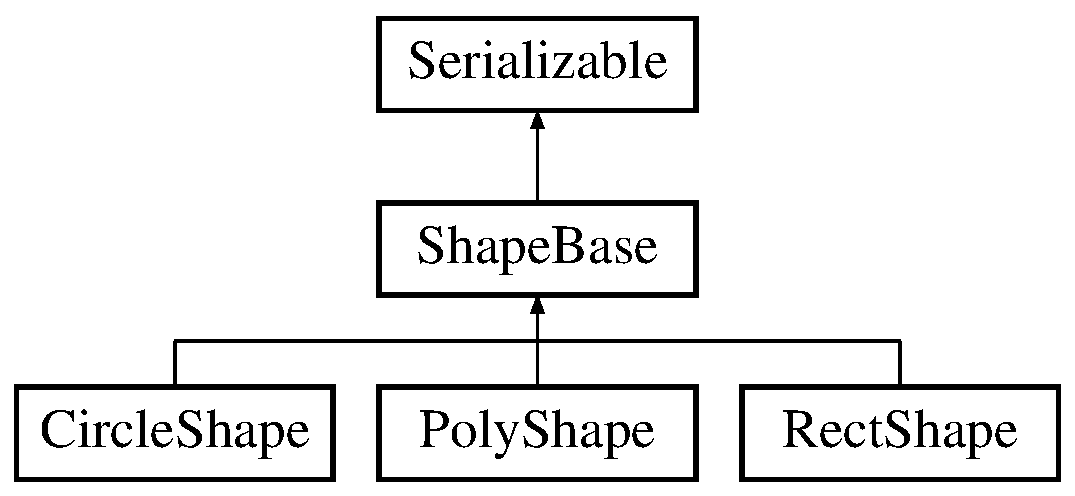
\includegraphics[height=3.000000cm]{class_shape_base}
\end{center}
\end{figure}
\subsection*{Public Member Functions}
\begin{DoxyCompactItemize}
\item 
abstract Shape \textbf{ get\+Shape} ()
\item 
abstract boolean \textbf{ is\+Hit} (float x, float y)
\item 
abstract void \textbf{ move} (int x, int y)
\item 
abstract void \textbf{ resize} (float value)
\item 
abstract void \textbf{ set\+Color} (Color new\+Color)
\item 
abstract Color \textbf{ get\+Color} ()
\end{DoxyCompactItemize}
\subsection*{Protected Attributes}
\begin{DoxyCompactItemize}
\item 
Color \textbf{ shape\+Color} = Color.\+R\+ED
\end{DoxyCompactItemize}


\subsection{Detailed Description}
Abstrakcyjna klasa odpowiedzialna za kształt figur. \begin{DoxyAuthor}{Author}
Michał Treter 
\end{DoxyAuthor}


\subsection{Member Function Documentation}
\mbox{\label{class_shape_base_aa2273c89bbd03d978c7a750293180fcb}} 
\index{Shape\+Base@{Shape\+Base}!get\+Color@{get\+Color}}
\index{get\+Color@{get\+Color}!Shape\+Base@{Shape\+Base}}
\subsubsection{get\+Color()}
{\footnotesize\ttfamily abstract Color Shape\+Base.\+get\+Color (\begin{DoxyParamCaption}{ }\end{DoxyParamCaption})\hspace{0.3cm}{\ttfamily [abstract]}}

Abstrakcyjna metoda zwracająca kolor kształtu. \begin{DoxyReturn}{Returns}
Aktualny kolor kształtu. 
\end{DoxyReturn}
\mbox{\label{class_shape_base_a0862131e56fc22f4315c01104f04b7c2}} 
\index{Shape\+Base@{Shape\+Base}!get\+Shape@{get\+Shape}}
\index{get\+Shape@{get\+Shape}!Shape\+Base@{Shape\+Base}}
\subsubsection{get\+Shape()}
{\footnotesize\ttfamily abstract Shape Shape\+Base.\+get\+Shape (\begin{DoxyParamCaption}{ }\end{DoxyParamCaption})\hspace{0.3cm}{\ttfamily [abstract]}}

Abstrakcyjna metoda zwracająca kształt figury. \begin{DoxyReturn}{Returns}
Kształt figury. 
\end{DoxyReturn}
\mbox{\label{class_shape_base_ac97cceedf62e85921e13a923599122dc}} 
\index{Shape\+Base@{Shape\+Base}!is\+Hit@{is\+Hit}}
\index{is\+Hit@{is\+Hit}!Shape\+Base@{Shape\+Base}}
\subsubsection{is\+Hit()}
{\footnotesize\ttfamily abstract boolean Shape\+Base.\+is\+Hit (\begin{DoxyParamCaption}\item[{float}]{x,  }\item[{float}]{y }\end{DoxyParamCaption})\hspace{0.3cm}{\ttfamily [abstract]}}

Abstrakcyjna metoda sprawdzając czy punkt znajduje się w kształcie. 
\begin{DoxyParams}{Parameters}
{\em x} & X punktu. \\
\hline
{\em y} & Y punktu. \\
\hline
\end{DoxyParams}
\begin{DoxyReturn}{Returns}
Wartość logiczna prawdziwa jeśli jest, fałszywa w przeciwnym wypadku. 
\end{DoxyReturn}
\mbox{\label{class_shape_base_a3408a350806c5e86336d6f628a46ad7c}} 
\index{Shape\+Base@{Shape\+Base}!move@{move}}
\index{move@{move}!Shape\+Base@{Shape\+Base}}
\subsubsection{move()}
{\footnotesize\ttfamily abstract void Shape\+Base.\+move (\begin{DoxyParamCaption}\item[{int}]{x,  }\item[{int}]{y }\end{DoxyParamCaption})\hspace{0.3cm}{\ttfamily [abstract]}}

Abstrakcyjna metoda przesuwająca kształt w osi X i osi Y. 
\begin{DoxyParams}{Parameters}
{\em x} & Wartość o ile przesunąć w osi X. \\
\hline
{\em y} & Wartość o ile przesunąć w osi X. \\
\hline
\end{DoxyParams}
\mbox{\label{class_shape_base_a0fc59d3f84903c188ac76c7d9648a2d2}} 
\index{Shape\+Base@{Shape\+Base}!resize@{resize}}
\index{resize@{resize}!Shape\+Base@{Shape\+Base}}
\subsubsection{resize()}
{\footnotesize\ttfamily abstract void Shape\+Base.\+resize (\begin{DoxyParamCaption}\item[{float}]{value }\end{DoxyParamCaption})\hspace{0.3cm}{\ttfamily [abstract]}}

Abstrakcyjna metoda zmieniająca rozmiar kształtu. 
\begin{DoxyParams}{Parameters}
{\em value} & Wartość o jaką zostaje zmniejszony rozmiar. \\
\hline
\end{DoxyParams}
\mbox{\label{class_shape_base_ac42b08e5966d3b53fbaa0ba077306fce}} 
\index{Shape\+Base@{Shape\+Base}!set\+Color@{set\+Color}}
\index{set\+Color@{set\+Color}!Shape\+Base@{Shape\+Base}}
\subsubsection{set\+Color()}
{\footnotesize\ttfamily abstract void Shape\+Base.\+set\+Color (\begin{DoxyParamCaption}\item[{Color}]{new\+Color }\end{DoxyParamCaption})\hspace{0.3cm}{\ttfamily [abstract]}}

Abstrakcyjna metoda zmieniająca kolor kształtu. 
\begin{DoxyParams}{Parameters}
{\em new\+Color} & Nowy kolor. \\
\hline
\end{DoxyParams}


\subsection{Member Data Documentation}
\mbox{\label{class_shape_base_aaf94f09219195ef803a3c6d2b67eca8e}} 
\index{Shape\+Base@{Shape\+Base}!shape\+Color@{shape\+Color}}
\index{shape\+Color@{shape\+Color}!Shape\+Base@{Shape\+Base}}
\subsubsection{shape\+Color}
{\footnotesize\ttfamily Color Shape\+Base.\+shape\+Color = Color.\+R\+ED\hspace{0.3cm}{\ttfamily [protected]}}

Kolor Figur. 

The documentation for this class was generated from the following file\+:\begin{DoxyCompactItemize}
\item 
/\+Users/\+Adimus/\+Desktop/\+N\+E\+T\+B\+I\+N\+Z/\+Geo\+Graphic\+X/src/Shape\+Base.\+java\end{DoxyCompactItemize}

\section{temp\+Circle Class Reference}
\label{classtemp_circle}\index{temp\+Circle@{temp\+Circle}}
Inheritance diagram for temp\+Circle\+:\begin{figure}[H]
\begin{center}
\leavevmode
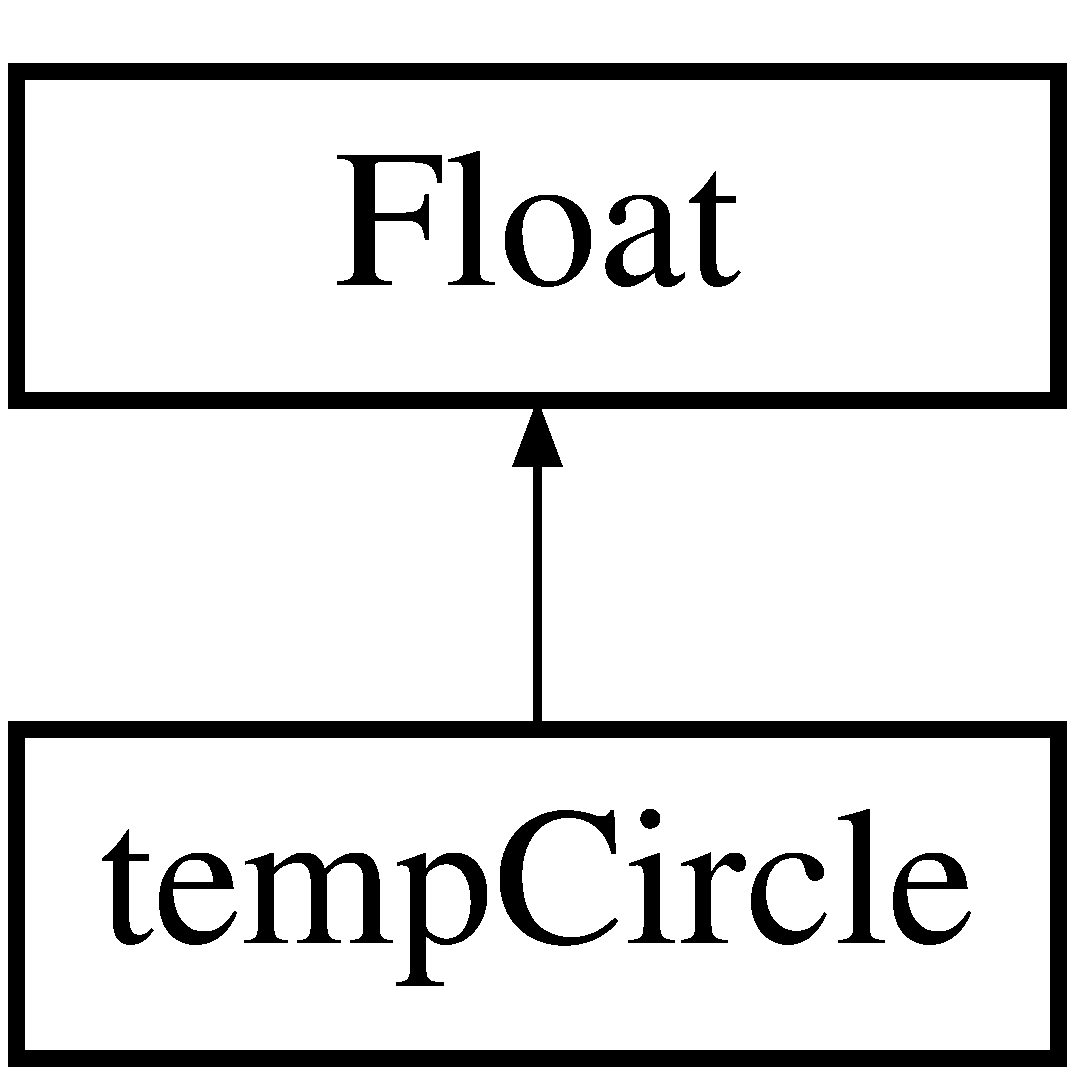
\includegraphics[height=2.000000cm]{classtemp_circle}
\end{center}
\end{figure}
\subsection*{Public Member Functions}
\begin{DoxyCompactItemize}
\item 
void \textbf{ set\+Position} (float x, float y)
\end{DoxyCompactItemize}


\subsection{Detailed Description}
\begin{DoxyAuthor}{Author}
adimus 
\end{DoxyAuthor}


\subsection{Member Function Documentation}
\mbox{\label{classtemp_circle_a5b1b7cc88f69197e8fdedbe5e74e312e}} 
\index{temp\+Circle@{temp\+Circle}!set\+Position@{set\+Position}}
\index{set\+Position@{set\+Position}!temp\+Circle@{temp\+Circle}}
\subsubsection{set\+Position()}
{\footnotesize\ttfamily void temp\+Circle.\+set\+Position (\begin{DoxyParamCaption}\item[{float}]{x,  }\item[{float}]{y }\end{DoxyParamCaption})}


\begin{DoxyParams}{Parameters}
{\em x} & \\
\hline
{\em y} & \\
\hline
\end{DoxyParams}


The documentation for this class was generated from the following file\+:\begin{DoxyCompactItemize}
\item 
/\+Users/\+Adimus/\+Desktop/\+N\+E\+T\+B\+I\+N\+Z/\+Geo\+Graphic\+X/src/temp\+Circle.\+java\end{DoxyCompactItemize}

\section{Utilities Class Reference}
\label{class_utilities}\index{Utilities@{Utilities}}
\subsection*{Static Public Member Functions}
\begin{DoxyCompactItemize}
\item 
static int \textbf{ find\+Lower} (int cord1, int cord2)
\item 
static int \textbf{ find\+Collision} (Array\+List$<$ \textbf{ Shape\+Base} $>$ given\+List, int cordX, int cordY)
\item 
static void \textbf{ save\+File} (\textbf{ Geo\+GraphicX} applet\+Reference, Array\+List$<$ \textbf{ Shape\+Base} $>$ given\+List)
\item 
static Array\+List$<$ \textbf{ Shape\+Base} $>$ \textbf{ load\+File} (\textbf{ Geo\+GraphicX} applet\+Reference)  throws Class\+Not\+Found\+Exception
\end{DoxyCompactItemize}


\subsection{Detailed Description}
Klasa zawierająca funkcje ułatwiające działanie programu. \begin{DoxyAuthor}{Author}
Michał Treter 
\end{DoxyAuthor}


\subsection{Member Function Documentation}
\mbox{\label{class_utilities_a65243cac27f1c4cc2d7f50e17915f942}} 
\index{Utilities@{Utilities}!find\+Collision@{find\+Collision}}
\index{find\+Collision@{find\+Collision}!Utilities@{Utilities}}
\subsubsection{find\+Collision()}
{\footnotesize\ttfamily static int Utilities.\+find\+Collision (\begin{DoxyParamCaption}\item[{Array\+List$<$ \textbf{ Shape\+Base} $>$}]{given\+List,  }\item[{int}]{cordX,  }\item[{int}]{cordY }\end{DoxyParamCaption})\hspace{0.3cm}{\ttfamily [static]}}

Funkcja znajdująca kolizję punktu kliknięcia z jedną z figur. 
\begin{DoxyParams}{Parameters}
{\em given\+List} & Lista figur. \\
\hline
{\em cordX} & X kliknięcia. \\
\hline
{\em cordY} & Y Kliknięcia. \\
\hline
\end{DoxyParams}
\begin{DoxyReturn}{Returns}
Numer elementu na liście z którym jest wykryta kolizja. Lub -\/1 kiedy jej nie ma. 
\end{DoxyReturn}
\mbox{\label{class_utilities_ac1e53d589e8d32c1fb0f920ebf01419f}} 
\index{Utilities@{Utilities}!find\+Lower@{find\+Lower}}
\index{find\+Lower@{find\+Lower}!Utilities@{Utilities}}
\subsubsection{find\+Lower()}
{\footnotesize\ttfamily static int Utilities.\+find\+Lower (\begin{DoxyParamCaption}\item[{int}]{cord1,  }\item[{int}]{cord2 }\end{DoxyParamCaption})\hspace{0.3cm}{\ttfamily [static]}}

Funkcja zwracająca mniejszą wartość. 
\begin{DoxyParams}{Parameters}
{\em cord1} & Wartość pierwsza. \\
\hline
{\em cord2} & Wartość druga. \\
\hline
\end{DoxyParams}
\begin{DoxyReturn}{Returns}
Mniejsza z tych wartości. 
\end{DoxyReturn}
\mbox{\label{class_utilities_affd5c9fd453405623493f7252deb1101}} 
\index{Utilities@{Utilities}!load\+File@{load\+File}}
\index{load\+File@{load\+File}!Utilities@{Utilities}}
\subsubsection{load\+File()}
{\footnotesize\ttfamily static Array\+List$<$\textbf{ Shape\+Base}$>$ Utilities.\+load\+File (\begin{DoxyParamCaption}\item[{\textbf{ Geo\+GraphicX}}]{applet\+Reference }\end{DoxyParamCaption}) throws Class\+Not\+Found\+Exception\hspace{0.3cm}{\ttfamily [static]}}

Funkcja wczytująca listę figur z pliku. 
\begin{DoxyParams}{Parameters}
{\em applet\+Reference} & Referencja do głównego apletu. \\
\hline
\end{DoxyParams}
\begin{DoxyReturn}{Returns}
Lista wczytana z pliku. 
\end{DoxyReturn}

\begin{DoxyExceptions}{Exceptions}
{\em Class\+Not\+Found\+Exception} & Wyjątek kiedy nastąpi niezgodność klas. \\
\hline
\end{DoxyExceptions}
\mbox{\label{class_utilities_a2e7fabe3109d97ded6a995c15657d487}} 
\index{Utilities@{Utilities}!save\+File@{save\+File}}
\index{save\+File@{save\+File}!Utilities@{Utilities}}
\subsubsection{save\+File()}
{\footnotesize\ttfamily static void Utilities.\+save\+File (\begin{DoxyParamCaption}\item[{\textbf{ Geo\+GraphicX}}]{applet\+Reference,  }\item[{Array\+List$<$ \textbf{ Shape\+Base} $>$}]{given\+List }\end{DoxyParamCaption})\hspace{0.3cm}{\ttfamily [static]}}

Funkcja eksportująca listę obiektów do pliku. 
\begin{DoxyParams}{Parameters}
{\em applet\+Reference} & Referencja do głównego apletu. \\
\hline
{\em given\+List} & Lista figur. \\
\hline
\end{DoxyParams}


The documentation for this class was generated from the following file\+:\begin{DoxyCompactItemize}
\item 
/\+Users/\+Adimus/\+Desktop/\+N\+E\+T\+B\+I\+N\+Z/\+Geo\+Graphic\+X/src/Utilities.\+java\end{DoxyCompactItemize}

%--- End generated contents ---

% Index
\backmatter
\newpage
\phantomsection
\clearemptydoublepage
\addcontentsline{toc}{chapter}{Index}
\printindex

\end{document}
